% Options for packages loaded elsewhere
\PassOptionsToPackage{unicode}{hyperref}
\PassOptionsToPackage{hyphens}{url}
\documentclass[
]{article}
\usepackage{xcolor}
\usepackage[margin=1in]{geometry}
\usepackage{amsmath,amssymb}
\setcounter{secnumdepth}{-\maxdimen} % remove section numbering
\usepackage{iftex}
\ifPDFTeX
  \usepackage[T1]{fontenc}
  \usepackage[utf8]{inputenc}
  \usepackage{textcomp} % provide euro and other symbols
\else % if luatex or xetex
  \usepackage{unicode-math} % this also loads fontspec
  \defaultfontfeatures{Scale=MatchLowercase}
  \defaultfontfeatures[\rmfamily]{Ligatures=TeX,Scale=1}
\fi
\usepackage{lmodern}
\ifPDFTeX\else
  % xetex/luatex font selection
\fi
% Use upquote if available, for straight quotes in verbatim environments
\IfFileExists{upquote.sty}{\usepackage{upquote}}{}
\IfFileExists{microtype.sty}{% use microtype if available
  \usepackage[]{microtype}
  \UseMicrotypeSet[protrusion]{basicmath} % disable protrusion for tt fonts
}{}
\makeatletter
\@ifundefined{KOMAClassName}{% if non-KOMA class
  \IfFileExists{parskip.sty}{%
    \usepackage{parskip}
  }{% else
    \setlength{\parindent}{0pt}
    \setlength{\parskip}{6pt plus 2pt minus 1pt}}
}{% if KOMA class
  \KOMAoptions{parskip=half}}
\makeatother
\usepackage{color}
\usepackage{fancyvrb}
\newcommand{\VerbBar}{|}
\newcommand{\VERB}{\Verb[commandchars=\\\{\}]}
\DefineVerbatimEnvironment{Highlighting}{Verbatim}{commandchars=\\\{\}}
% Add ',fontsize=\small' for more characters per line
\usepackage{framed}
\definecolor{shadecolor}{RGB}{248,248,248}
\newenvironment{Shaded}{\begin{snugshade}}{\end{snugshade}}
\newcommand{\AlertTok}[1]{\textcolor[rgb]{0.94,0.16,0.16}{#1}}
\newcommand{\AnnotationTok}[1]{\textcolor[rgb]{0.56,0.35,0.01}{\textbf{\textit{#1}}}}
\newcommand{\AttributeTok}[1]{\textcolor[rgb]{0.13,0.29,0.53}{#1}}
\newcommand{\BaseNTok}[1]{\textcolor[rgb]{0.00,0.00,0.81}{#1}}
\newcommand{\BuiltInTok}[1]{#1}
\newcommand{\CharTok}[1]{\textcolor[rgb]{0.31,0.60,0.02}{#1}}
\newcommand{\CommentTok}[1]{\textcolor[rgb]{0.56,0.35,0.01}{\textit{#1}}}
\newcommand{\CommentVarTok}[1]{\textcolor[rgb]{0.56,0.35,0.01}{\textbf{\textit{#1}}}}
\newcommand{\ConstantTok}[1]{\textcolor[rgb]{0.56,0.35,0.01}{#1}}
\newcommand{\ControlFlowTok}[1]{\textcolor[rgb]{0.13,0.29,0.53}{\textbf{#1}}}
\newcommand{\DataTypeTok}[1]{\textcolor[rgb]{0.13,0.29,0.53}{#1}}
\newcommand{\DecValTok}[1]{\textcolor[rgb]{0.00,0.00,0.81}{#1}}
\newcommand{\DocumentationTok}[1]{\textcolor[rgb]{0.56,0.35,0.01}{\textbf{\textit{#1}}}}
\newcommand{\ErrorTok}[1]{\textcolor[rgb]{0.64,0.00,0.00}{\textbf{#1}}}
\newcommand{\ExtensionTok}[1]{#1}
\newcommand{\FloatTok}[1]{\textcolor[rgb]{0.00,0.00,0.81}{#1}}
\newcommand{\FunctionTok}[1]{\textcolor[rgb]{0.13,0.29,0.53}{\textbf{#1}}}
\newcommand{\ImportTok}[1]{#1}
\newcommand{\InformationTok}[1]{\textcolor[rgb]{0.56,0.35,0.01}{\textbf{\textit{#1}}}}
\newcommand{\KeywordTok}[1]{\textcolor[rgb]{0.13,0.29,0.53}{\textbf{#1}}}
\newcommand{\NormalTok}[1]{#1}
\newcommand{\OperatorTok}[1]{\textcolor[rgb]{0.81,0.36,0.00}{\textbf{#1}}}
\newcommand{\OtherTok}[1]{\textcolor[rgb]{0.56,0.35,0.01}{#1}}
\newcommand{\PreprocessorTok}[1]{\textcolor[rgb]{0.56,0.35,0.01}{\textit{#1}}}
\newcommand{\RegionMarkerTok}[1]{#1}
\newcommand{\SpecialCharTok}[1]{\textcolor[rgb]{0.81,0.36,0.00}{\textbf{#1}}}
\newcommand{\SpecialStringTok}[1]{\textcolor[rgb]{0.31,0.60,0.02}{#1}}
\newcommand{\StringTok}[1]{\textcolor[rgb]{0.31,0.60,0.02}{#1}}
\newcommand{\VariableTok}[1]{\textcolor[rgb]{0.00,0.00,0.00}{#1}}
\newcommand{\VerbatimStringTok}[1]{\textcolor[rgb]{0.31,0.60,0.02}{#1}}
\newcommand{\WarningTok}[1]{\textcolor[rgb]{0.56,0.35,0.01}{\textbf{\textit{#1}}}}
\usepackage{longtable,booktabs,array}
\usepackage{calc} % for calculating minipage widths
% Correct order of tables after \paragraph or \subparagraph
\usepackage{etoolbox}
\makeatletter
\patchcmd\longtable{\par}{\if@noskipsec\mbox{}\fi\par}{}{}
\makeatother
% Allow footnotes in longtable head/foot
\IfFileExists{footnotehyper.sty}{\usepackage{footnotehyper}}{\usepackage{footnote}}
\makesavenoteenv{longtable}
\usepackage{graphicx}
\makeatletter
\newsavebox\pandoc@box
\newcommand*\pandocbounded[1]{% scales image to fit in text height/width
  \sbox\pandoc@box{#1}%
  \Gscale@div\@tempa{\textheight}{\dimexpr\ht\pandoc@box+\dp\pandoc@box\relax}%
  \Gscale@div\@tempb{\linewidth}{\wd\pandoc@box}%
  \ifdim\@tempb\p@<\@tempa\p@\let\@tempa\@tempb\fi% select the smaller of both
  \ifdim\@tempa\p@<\p@\scalebox{\@tempa}{\usebox\pandoc@box}%
  \else\usebox{\pandoc@box}%
  \fi%
}
% Set default figure placement to htbp
\def\fps@figure{htbp}
\makeatother
\setlength{\emergencystretch}{3em} % prevent overfull lines
\providecommand{\tightlist}{%
  \setlength{\itemsep}{0pt}\setlength{\parskip}{0pt}}
\usepackage{bookmark}
\IfFileExists{xurl.sty}{\usepackage{xurl}}{} % add URL line breaks if available
\urlstyle{same}
\hypersetup{
  pdftitle={BANA4040 Predictive Analytics},
  pdfauthor={Phan Nu Quynh Huong},
  hidelinks,
  pdfcreator={LaTeX via pandoc}}

\title{BANA4040 Predictive Analytics}
\author{Phan Nu Quynh Huong}
\date{2025-03-12}

\begin{document}
\maketitle

\subsection{Problem 1}\label{problem-1}

In this problem, we will perform model selection in R. The data used for
this problem is stored in ``data.xlsx''. In the related study, a
personnel officer in a governmental agency administered four Assignment
№ 1 Page 1 newly developed aptitude tests to each of 25 applicants for
entry-level clerical positions in the agency. For purpose of the study,
all 25 applicants were accepted for positions irrespective of their test
scores. After a probationary period, each applicant was rated for
proficiency on the job. The data file include the job proficiency score
(y, the first column) and scores on the four tests (refer as t1;t2;t3;t4
thereafter). As there are no column headers for this data file, so be
sure to assign appropriate column headings for the dataframe after
import.

\subsection{Part 1}\label{part-1}

Graphical summaries: Before performing any of the model selection
techniques, it is always a good idea to generate some graphical
summaries of the data. For example, scatterplots of the response
variable proficiency against each predictor individually. What do these
plots suggest? \#\# Load Data

\begin{Shaded}
\begin{Highlighting}[]
\CommentTok{\# Sử dụng thư viện readxl để đọc dữ liệu từ file Excel}
\FunctionTok{library}\NormalTok{(readxl)}

\CommentTok{\# Đọc dữ liệu từ file "data.xlsx" }
\CommentTok{\# Tham số col\_names = FALSE có nghĩa là file không có hàng tiêu đề nên chúng ta sẽ tự đặt tên sau này.}
\NormalTok{jobs }\OtherTok{\textless{}{-}} \FunctionTok{read\_excel}\NormalTok{(}\StringTok{"data.xlsx"}\NormalTok{, }\AttributeTok{col\_names =} \ConstantTok{FALSE}\NormalTok{)}
\CommentTok{\#\textgreater{} New names:}
\CommentTok{\#\textgreater{} * \textasciigrave{}\textasciigrave{} {-}\textgreater{} \textasciigrave{}...1\textasciigrave{}}
\CommentTok{\#\textgreater{} * \textasciigrave{}\textasciigrave{} {-}\textgreater{} \textasciigrave{}...2\textasciigrave{}}
\CommentTok{\#\textgreater{} * \textasciigrave{}\textasciigrave{} {-}\textgreater{} \textasciigrave{}...3\textasciigrave{}}
\CommentTok{\#\textgreater{} * \textasciigrave{}\textasciigrave{} {-}\textgreater{} \textasciigrave{}...4\textasciigrave{}}
\CommentTok{\#\textgreater{} * \textasciigrave{}\textasciigrave{} {-}\textgreater{} \textasciigrave{}...5\textasciigrave{}}

\CommentTok{\# Gán tên cho các cột của dataframe:}
\CommentTok{\# {-} "proficiency": độ chuyên môn của công việc}
\CommentTok{\# {-} "t1", "t2", "t3", "t4": điểm số của các bài kiểm tra tương ứng.}
\FunctionTok{colnames}\NormalTok{(jobs) }\OtherTok{\textless{}{-}} \FunctionTok{c}\NormalTok{(}\StringTok{"proficiency"}\NormalTok{, }\StringTok{"t1"}\NormalTok{, }\StringTok{"t2"}\NormalTok{, }\StringTok{"t3"}\NormalTok{, }\StringTok{"t4"}\NormalTok{)}

\CommentTok{\# Hiển thị tóm tắt thống kê của dữ liệu (bao gồm min, max, median, mean, ...)}
\FunctionTok{summary}\NormalTok{(jobs)}
\CommentTok{\#\textgreater{}   proficiency          t1              t2              t3       }
\CommentTok{\#\textgreater{}  Min.   : 58.0   Min.   : 62.0   Min.   : 73.0   Min.   : 80.0  }
\CommentTok{\#\textgreater{}  1st Qu.: 78.0   1st Qu.: 91.0   1st Qu.: 94.0   1st Qu.: 95.0  }
\CommentTok{\#\textgreater{}  Median : 94.0   Median :104.0   Median :113.0   Median :100.0  }
\CommentTok{\#\textgreater{}  Mean   : 92.2   Mean   :103.4   Mean   :106.7   Mean   :100.8  }
\CommentTok{\#\textgreater{}  3rd Qu.:109.0   3rd Qu.:112.0   3rd Qu.:121.0   3rd Qu.:107.0  }
\CommentTok{\#\textgreater{}  Max.   :127.0   Max.   :150.0   Max.   :129.0   Max.   :116.0  }
\CommentTok{\#\textgreater{}        t4        }
\CommentTok{\#\textgreater{}  Min.   : 74.00  }
\CommentTok{\#\textgreater{}  1st Qu.: 87.00  }
\CommentTok{\#\textgreater{}  Median : 95.00  }
\CommentTok{\#\textgreater{}  Mean   : 94.68  }
\CommentTok{\#\textgreater{}  3rd Qu.:103.00  }
\CommentTok{\#\textgreater{}  Max.   :110.00}
\end{Highlighting}
\end{Shaded}

\subsection{Visualize Data}\label{visualize-data}

We create scatterplots to visualize the relationship between job
proficiency and each test score.

\begin{Shaded}
\begin{Highlighting}[]
\CommentTok{\# Thiết lập kích thước biểu đồ để hiển thị rõ ràng}
\FunctionTok{options}\NormalTok{(}\AttributeTok{repr.plot.width =} \DecValTok{20}\NormalTok{, }\AttributeTok{repr.plot.height =} \DecValTok{20}\NormalTok{)}

\CommentTok{\# Chia vùng vẽ thành 2 hàng x 2 cột để hiển thị 4 biểu đồ cùng lúc.}
\CommentTok{\# Tham số mfrow = c(2, 2) điều chỉnh lưới vẽ biểu đồ.}
\CommentTok{\# Tham số mar = c(4, 4, 2, 1) thiết lập lề (margin) cho biểu đồ: dưới, trái, trên, phải.}
\FunctionTok{par}\NormalTok{(}\AttributeTok{mfrow =} \FunctionTok{c}\NormalTok{(}\DecValTok{2}\NormalTok{, }\DecValTok{2}\NormalTok{), }\AttributeTok{mar =} \FunctionTok{c}\NormalTok{(}\DecValTok{4}\NormalTok{, }\DecValTok{4}\NormalTok{, }\DecValTok{2}\NormalTok{, }\DecValTok{1}\NormalTok{))}

\CommentTok{\# Biểu đồ phân tán: điểm số Test 1 (t1) vs độ chuyên môn (proficiency)}
\FunctionTok{plot}\NormalTok{(jobs}\SpecialCharTok{$}\NormalTok{t1, jobs}\SpecialCharTok{$}\NormalTok{proficiency,}
     \AttributeTok{xlab =} \StringTok{"Test 1 (t1)"}\NormalTok{,      }\CommentTok{\# Nhãn trục X: điểm của bài kiểm tra t1}
     \AttributeTok{ylab =} \StringTok{"Job Proficiency"}\NormalTok{,  }\CommentTok{\# Nhãn trục Y: độ chuyên môn}
     \AttributeTok{main =} \StringTok{"Proficiency vs t1"}\NormalTok{)}\CommentTok{\# Tiêu đề biểu đồ}

\CommentTok{\# Biểu đồ phân tán: điểm số Test 2 (t2) vs độ chuyên môn}
\FunctionTok{plot}\NormalTok{(jobs}\SpecialCharTok{$}\NormalTok{t2, jobs}\SpecialCharTok{$}\NormalTok{proficiency,}
     \AttributeTok{xlab =} \StringTok{"Test 2 (t2)"}\NormalTok{,}
     \AttributeTok{ylab =} \StringTok{"Job Proficiency"}\NormalTok{,}
     \AttributeTok{main =} \StringTok{"Proficiency vs t2"}\NormalTok{)}

\CommentTok{\# Biểu đồ phân tán: điểm số Test 3 (t3) vs độ chuyên môn}
\FunctionTok{plot}\NormalTok{(jobs}\SpecialCharTok{$}\NormalTok{t3, jobs}\SpecialCharTok{$}\NormalTok{proficiency,}
     \AttributeTok{xlab =} \StringTok{"Test 3 (t3)"}\NormalTok{,}
     \AttributeTok{ylab =} \StringTok{"Job Proficiency"}\NormalTok{,}
     \AttributeTok{main =} \StringTok{"Proficiency vs t3"}\NormalTok{)}

\CommentTok{\# Biểu đồ phân tán: điểm số Test 4 (t4) vs độ chuyên môn}
\FunctionTok{plot}\NormalTok{(jobs}\SpecialCharTok{$}\NormalTok{t4, jobs}\SpecialCharTok{$}\NormalTok{proficiency,}
     \AttributeTok{xlab =} \StringTok{"Test 4 (t4)"}\NormalTok{,}
     \AttributeTok{ylab =} \StringTok{"Job Proficiency"}\NormalTok{,}
     \AttributeTok{main =} \StringTok{"Proficiency vs t4"}\NormalTok{)}
\end{Highlighting}
\end{Shaded}

\pandocbounded{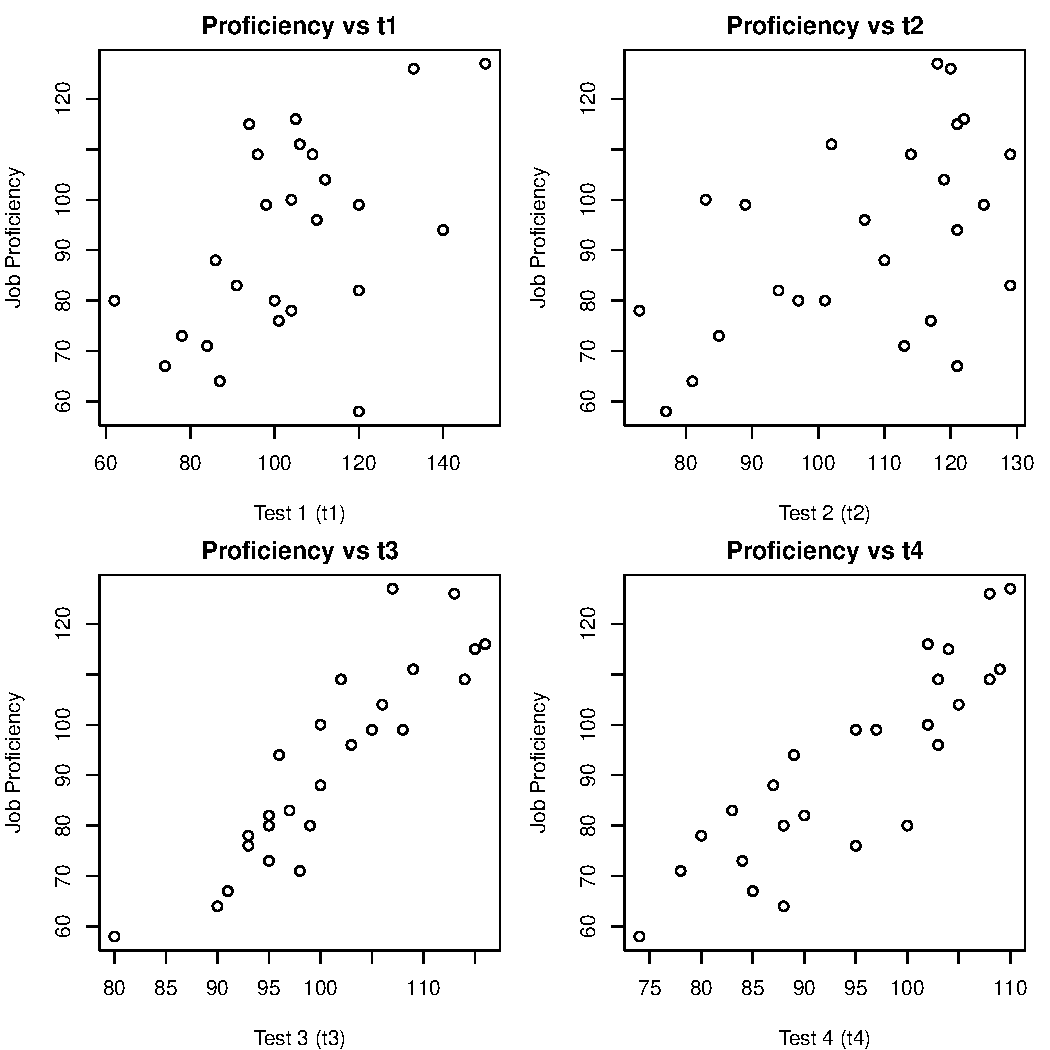
\includegraphics[keepaspectratio]{RMD_files/figure-latex/scatterplots-1.pdf}}

\begin{Shaded}
\begin{Highlighting}[]

\CommentTok{\# Sau khi hoàn thành vẽ 4 biểu đồ, đặt lại vùng vẽ về mặc định (1 hàng, 1 cột)}
\FunctionTok{par}\NormalTok{(}\AttributeTok{mfrow =} \FunctionTok{c}\NormalTok{(}\DecValTok{1}\NormalTok{, }\DecValTok{1}\NormalTok{))}
\end{Highlighting}
\end{Shaded}

\subsection{Conclusion}\label{conclusion}

From a quick visual inspection, the plots suggest that both t3 and t4
have a relatively strong, positively sloped relationship with the
proficiency measure (i.e., as the test scores go up, so does
proficiency, and the points fall roughly along a line). By contrast, t1
and t2 still appear to be positively correlated with proficiency but not
as strongly or as cleanly as t3 and t4.

In more detail:

t1 vs.~proficiency: The points show a positive trend overall, but the
relationship looks fairly scattered. There is some upward slope, yet
more variability around the trend line compared to t3 and t4.

t2 vs.~proficiency: Similar to t1, there is an upward trend but it is
not as tight.

t3 vs.~proficiency: The scatterplot indicates a strong, roughly linear
relationship: as t3 increases, proficiency tends to increase in a fairly
straight line.

t4 vs.~proficiency: The points also exhibit a clear, strong positive
trend, though perhaps with slightly more spread than t3.

In short, the plots suggest that t3 and t4 are likely to be the
strongest individual predictors of proficiency, whereas t1 and t2 show
weaker but still positive relationships.

\subsection{Part 2}\label{part-2}

Performing all possible regressions: Follow the steps of the code in
class, fit all possible regression models (4 predictors will generate 16
different models). For each model, record the following information for
model selection purpose: p, number of parameters, R2, R2a,p,P RESSp,
AICp, BICp, and Mallows Cp

\begin{Shaded}
\begin{Highlighting}[]

\NormalTok{model\_stats }\OtherTok{\textless{}{-}} \ControlFlowTok{function}\NormalTok{(fit, MSE\_full)\{}
  \CommentTok{\# fit: đối tượng lm (mô hình hồi quy)}
  \CommentTok{\# MSE\_full: Mean Squared Error của mô hình đầy đủ dùng để tính Mallows\textquotesingle{} Cp}
  
\NormalTok{  n }\OtherTok{\textless{}{-}} \FunctionTok{length}\NormalTok{(fit}\SpecialCharTok{$}\NormalTok{residuals)    }\CommentTok{\# Số lượng quan sát}
\NormalTok{  p }\OtherTok{\textless{}{-}} \FunctionTok{length}\NormalTok{(}\FunctionTok{coef}\NormalTok{(fit))        }\CommentTok{\# Số tham số (bao gồm intercept)}
  
  \CommentTok{\# Tính hệ số xác định R² và R² hiệu chỉnh từ kết quả summary của mô hình}
\NormalTok{  r2     }\OtherTok{\textless{}{-}} \FunctionTok{summary}\NormalTok{(fit)}\SpecialCharTok{$}\NormalTok{r.squared}
\NormalTok{  adjr2  }\OtherTok{\textless{}{-}} \FunctionTok{summary}\NormalTok{(fit)}\SpecialCharTok{$}\NormalTok{adj.r.squared}
  
  \CommentTok{\# Tính tổng bình phương sai số (SSE) của mô hình fit}
\NormalTok{  sse\_p  }\OtherTok{\textless{}{-}} \FunctionTok{sum}\NormalTok{(}\FunctionTok{resid}\NormalTok{(fit)}\SpecialCharTok{\^{}}\DecValTok{2}\NormalTok{)}
  
  \CommentTok{\# Tính chỉ số PRESS: PRESS = Σ[(e\_i / (1 {-} h\_ii))\^{}2]}
  \CommentTok{\# Trong đó: e\_i là phần dư, h\_ii là giá trị hat (đo lường ảnh hưởng của mỗi quan sát)}
\NormalTok{  hat    }\OtherTok{\textless{}{-}} \FunctionTok{lm.influence}\NormalTok{(fit)}\SpecialCharTok{$}\NormalTok{hat  }\CommentTok{\# Lấy giá trị hat của mô hình}
\NormalTok{  res    }\OtherTok{\textless{}{-}} \FunctionTok{resid}\NormalTok{(fit)            }\CommentTok{\# Lấy phần dư của mô hình}
\NormalTok{  press  }\OtherTok{\textless{}{-}} \FunctionTok{sum}\NormalTok{((res}\SpecialCharTok{/}\NormalTok{(}\DecValTok{1} \SpecialCharTok{{-}}\NormalTok{ hat))}\SpecialCharTok{\^{}}\DecValTok{2}\NormalTok{)}
  
  \CommentTok{\# Tính AIC và BIC của mô hình}
\NormalTok{  aic\_val }\OtherTok{\textless{}{-}} \FunctionTok{AIC}\NormalTok{(fit)}
\NormalTok{  bic\_val }\OtherTok{\textless{}{-}} \FunctionTok{BIC}\NormalTok{(fit)}
  
  \CommentTok{\# Tính Mallows\textquotesingle{} Cp với công thức: Cp = SSE\_p / MSE\_full {-} (n {-} 2*p)}
\NormalTok{  cp\_val  }\OtherTok{\textless{}{-}}\NormalTok{ sse\_p }\SpecialCharTok{/}\NormalTok{ MSE\_full }\SpecialCharTok{{-}}\NormalTok{ (n }\SpecialCharTok{{-}} \DecValTok{2}\SpecialCharTok{*}\NormalTok{p)}
  
  \CommentTok{\# Trả về vector chứa các chỉ số}
  \FunctionTok{return}\NormalTok{(}\FunctionTok{c}\NormalTok{(p, r2, adjr2, press, aic\_val, bic\_val, cp\_val))}
\NormalTok{\}}
\end{Highlighting}
\end{Shaded}

\begin{Shaded}
\begin{Highlighting}[]
\CommentTok{\# Xây dựng mô hình hồi quy đầy đủ với tất cả các biến dự báo}
\NormalTok{lm\_full }\OtherTok{\textless{}{-}} \FunctionTok{lm}\NormalTok{(proficiency }\SpecialCharTok{\textasciitilde{}}\NormalTok{ t1 }\SpecialCharTok{+}\NormalTok{ t2 }\SpecialCharTok{+}\NormalTok{ t3 }\SpecialCharTok{+}\NormalTok{ t4, }\AttributeTok{data =}\NormalTok{ jobs)}

\CommentTok{\# Tính tổng bình phương sai số (SSE) của mô hình đầy đủ}
\NormalTok{SSE\_full }\OtherTok{\textless{}{-}} \FunctionTok{sum}\NormalTok{(}\FunctionTok{resid}\NormalTok{(lm\_full)}\SpecialCharTok{\^{}}\DecValTok{2}\NormalTok{)}

\CommentTok{\# Số lượng quan sát trong dữ liệu}
\NormalTok{n }\OtherTok{\textless{}{-}} \FunctionTok{nrow}\NormalTok{(jobs)}

\CommentTok{\# Số tham số của mô hình đầy đủ (4 biến dự báo + intercept)}
\NormalTok{p\_full }\OtherTok{\textless{}{-}} \FunctionTok{length}\NormalTok{(}\FunctionTok{coef}\NormalTok{(lm\_full)) }

\CommentTok{\# Tính Mean Squared Error (MSE) của mô hình đầy đủ}
\NormalTok{MSE\_full }\OtherTok{\textless{}{-}}\NormalTok{ SSE\_full }\SpecialCharTok{/}\NormalTok{ (n }\SpecialCharTok{{-}}\NormalTok{ p\_full)}
\end{Highlighting}
\end{Shaded}

\begin{Shaded}
\begin{Highlighting}[]
\CommentTok{\# Tạo dataframe rỗng để lưu kết quả}
\NormalTok{results }\OtherTok{\textless{}{-}} \FunctionTok{data.frame}\NormalTok{(}
  \AttributeTok{Model   =} \FunctionTok{character}\NormalTok{(),}
  \AttributeTok{p       =} \FunctionTok{numeric}\NormalTok{(),  }\CommentTok{\# Số tham số (bao gồm intercept)}
  \AttributeTok{R2      =} \FunctionTok{numeric}\NormalTok{(),}
  \AttributeTok{AdjR2   =} \FunctionTok{numeric}\NormalTok{(),}
  \AttributeTok{PRESS   =} \FunctionTok{numeric}\NormalTok{(),}
  \AttributeTok{AIC     =} \FunctionTok{numeric}\NormalTok{(),}
  \AttributeTok{BIC     =} \FunctionTok{numeric}\NormalTok{(),}
  \AttributeTok{Cp      =} \FunctionTok{numeric}\NormalTok{(),}
  \AttributeTok{stringsAsFactors =} \ConstantTok{FALSE}
\NormalTok{)}

\CommentTok{\# Danh sách các biến dự báo}
\NormalTok{preds }\OtherTok{\textless{}{-}} \FunctionTok{c}\NormalTok{(}\StringTok{"t1"}\NormalTok{, }\StringTok{"t2"}\NormalTok{, }\StringTok{"t3"}\NormalTok{, }\StringTok{"t4"}\NormalTok{)}

\CommentTok{\# Duyệt qua các tập con của biến dự báo với số lượng biến từ 0 đến 4}
\ControlFlowTok{for}\NormalTok{ (k }\ControlFlowTok{in} \DecValTok{0}\SpecialCharTok{:}\DecValTok{4}\NormalTok{) \{}
  \CommentTok{\# Lấy tất cả tổ hợp k phần tử từ vector preds}
\NormalTok{  subset\_list }\OtherTok{\textless{}{-}} \FunctionTok{combn}\NormalTok{(preds, k)}
  
  \ControlFlowTok{if}\NormalTok{ (k }\SpecialCharTok{==} \DecValTok{0}\NormalTok{) \{}
    \CommentTok{\# Trường hợp k = 0: mô hình chỉ có intercept (không có biến dự báo)}
\NormalTok{    form }\OtherTok{\textless{}{-}} \FunctionTok{as.formula}\NormalTok{(}\StringTok{"proficiency \textasciitilde{} 1"}\NormalTok{)}
\NormalTok{    fit }\OtherTok{\textless{}{-}} \FunctionTok{lm}\NormalTok{(form, }\AttributeTok{data =}\NormalTok{ jobs)}
\NormalTok{    stats }\OtherTok{\textless{}{-}} \FunctionTok{model\_stats}\NormalTok{(fit, MSE\_full)}
    
\NormalTok{    results }\OtherTok{\textless{}{-}} \FunctionTok{rbind}\NormalTok{(}
\NormalTok{      results,}
      \FunctionTok{data.frame}\NormalTok{(}
        \AttributeTok{Model =} \StringTok{"Intercept Only"}\NormalTok{,}
        \AttributeTok{p     =}\NormalTok{ stats[}\DecValTok{1}\NormalTok{],}
        \AttributeTok{R2    =}\NormalTok{ stats[}\DecValTok{2}\NormalTok{],}
        \AttributeTok{AdjR2 =}\NormalTok{ stats[}\DecValTok{3}\NormalTok{],}
        \AttributeTok{PRESS =}\NormalTok{ stats[}\DecValTok{4}\NormalTok{],}
        \AttributeTok{AIC   =}\NormalTok{ stats[}\DecValTok{5}\NormalTok{],}
        \AttributeTok{BIC   =}\NormalTok{ stats[}\DecValTok{6}\NormalTok{],}
        \AttributeTok{Cp    =}\NormalTok{ stats[}\DecValTok{7}\NormalTok{],}
        \AttributeTok{stringsAsFactors =} \ConstantTok{FALSE}
\NormalTok{      )}
\NormalTok{    )}
    
\NormalTok{  \} }\ControlFlowTok{else}\NormalTok{ \{}
    \CommentTok{\# Trường hợp k \textgreater{} 0: duyệt qua từng tổ hợp của các biến dự báo}
    \ControlFlowTok{for}\NormalTok{ (i }\ControlFlowTok{in} \DecValTok{1}\SpecialCharTok{:}\FunctionTok{ncol}\NormalTok{(subset\_list)) \{}
\NormalTok{      vars }\OtherTok{\textless{}{-}}\NormalTok{ subset\_list[, i]  }\CommentTok{\# Lấy tập hợp các biến dự báo cho mô hình hiện tại}
      
      \CommentTok{\# Tạo công thức hồi quy từ các biến được chọn}
\NormalTok{      form }\OtherTok{\textless{}{-}} \FunctionTok{as.formula}\NormalTok{(}\FunctionTok{paste}\NormalTok{(}\StringTok{"proficiency \textasciitilde{}"}\NormalTok{, }\FunctionTok{paste}\NormalTok{(vars, }\AttributeTok{collapse =} \StringTok{" + "}\NormalTok{)))}
      
      \CommentTok{\# Xây dựng mô hình hồi quy với công thức trên}
\NormalTok{      fit }\OtherTok{\textless{}{-}} \FunctionTok{lm}\NormalTok{(form, }\AttributeTok{data =}\NormalTok{ jobs)}
\NormalTok{      stats }\OtherTok{\textless{}{-}} \FunctionTok{model\_stats}\NormalTok{(fit, MSE\_full)}
      
      \CommentTok{\# Thêm kết quả của mô hình vào dataframe results}
\NormalTok{      results }\OtherTok{\textless{}{-}} \FunctionTok{rbind}\NormalTok{(}
\NormalTok{        results,}
        \FunctionTok{data.frame}\NormalTok{(}
          \AttributeTok{Model =} \FunctionTok{paste}\NormalTok{(vars, }\AttributeTok{collapse =} \StringTok{" + "}\NormalTok{),}
          \AttributeTok{p     =}\NormalTok{ stats[}\DecValTok{1}\NormalTok{],}
          \AttributeTok{R2    =}\NormalTok{ stats[}\DecValTok{2}\NormalTok{],}
          \AttributeTok{AdjR2 =}\NormalTok{ stats[}\DecValTok{3}\NormalTok{],}
          \AttributeTok{PRESS =}\NormalTok{ stats[}\DecValTok{4}\NormalTok{],}
          \AttributeTok{AIC   =}\NormalTok{ stats[}\DecValTok{5}\NormalTok{],}
          \AttributeTok{BIC   =}\NormalTok{ stats[}\DecValTok{6}\NormalTok{],}
          \AttributeTok{Cp    =}\NormalTok{ stats[}\DecValTok{7}\NormalTok{],}
          \AttributeTok{stringsAsFactors =} \ConstantTok{FALSE}
\NormalTok{        )}
\NormalTok{      )}
\NormalTok{    \}}
\NormalTok{  \}}
\NormalTok{\}}
\end{Highlighting}
\end{Shaded}

\begin{Shaded}
\begin{Highlighting}[]
\CommentTok{\# In kết quả các chỉ số thống kê của các mô hình con}
\NormalTok{knitr}\SpecialCharTok{::}\FunctionTok{kable}\NormalTok{(results, }\AttributeTok{caption =} \StringTok{"Bảng kết quả các mô hình dự báo"}\NormalTok{)}
\end{Highlighting}
\end{Shaded}

\begin{longtable}[]{@{}
  >{\raggedright\arraybackslash}p{(\linewidth - 14\tabcolsep) * \real{0.2250}}
  >{\raggedleft\arraybackslash}p{(\linewidth - 14\tabcolsep) * \real{0.0375}}
  >{\raggedleft\arraybackslash}p{(\linewidth - 14\tabcolsep) * \real{0.1250}}
  >{\raggedleft\arraybackslash}p{(\linewidth - 14\tabcolsep) * \real{0.1250}}
  >{\raggedleft\arraybackslash}p{(\linewidth - 14\tabcolsep) * \real{0.1250}}
  >{\raggedleft\arraybackslash}p{(\linewidth - 14\tabcolsep) * \real{0.1125}}
  >{\raggedleft\arraybackslash}p{(\linewidth - 14\tabcolsep) * \real{0.1125}}
  >{\raggedleft\arraybackslash}p{(\linewidth - 14\tabcolsep) * \real{0.1375}}@{}}
\caption{Bảng kết quả các mô hình dự báo}\tabularnewline
\toprule\noalign{}
\begin{minipage}[b]{\linewidth}\raggedright
Model
\end{minipage} & \begin{minipage}[b]{\linewidth}\raggedleft
p
\end{minipage} & \begin{minipage}[b]{\linewidth}\raggedleft
R2
\end{minipage} & \begin{minipage}[b]{\linewidth}\raggedleft
AdjR2
\end{minipage} & \begin{minipage}[b]{\linewidth}\raggedleft
PRESS
\end{minipage} & \begin{minipage}[b]{\linewidth}\raggedleft
AIC
\end{minipage} & \begin{minipage}[b]{\linewidth}\raggedleft
BIC
\end{minipage} & \begin{minipage}[b]{\linewidth}\raggedleft
Cp
\end{minipage} \\
\midrule\noalign{}
\endfirsthead
\toprule\noalign{}
\begin{minipage}[b]{\linewidth}\raggedright
Model
\end{minipage} & \begin{minipage}[b]{\linewidth}\raggedleft
p
\end{minipage} & \begin{minipage}[b]{\linewidth}\raggedleft
R2
\end{minipage} & \begin{minipage}[b]{\linewidth}\raggedleft
AdjR2
\end{minipage} & \begin{minipage}[b]{\linewidth}\raggedleft
PRESS
\end{minipage} & \begin{minipage}[b]{\linewidth}\raggedleft
AIC
\end{minipage} & \begin{minipage}[b]{\linewidth}\raggedleft
BIC
\end{minipage} & \begin{minipage}[b]{\linewidth}\raggedleft
Cp
\end{minipage} \\
\midrule\noalign{}
\endhead
\bottomrule\noalign{}
\endlastfoot
Intercept Only & 1 & 0.0000000 & 0.0000000 & 9824.2188 & 222.2491 &
224.6868 & 515.964627 \\
t1 & 2 & 0.2646184 & 0.2326452 & 7791.5994 & 216.5649 & 220.2216 &
375.344689 \\
t2 & 2 & 0.2470147 & 0.2142762 & 7991.0964 & 217.1563 & 220.8130 &
384.832454 \\
t3 & 2 & 0.8047247 & 0.7962344 & 2064.5976 & 183.4155 & 187.0721 &
84.246496 \\
t4 & 2 & 0.7558329 & 0.7452170 & 2548.6349 & 189.0015 & 192.6581 &
110.597414 \\
t1 + t2 & 3 & 0.4641948 & 0.4154853 & 6444.0411 & 210.6495 & 215.5250 &
269.780029 \\
t1 + t3 & 3 & 0.9329956 & 0.9269043 & 760.9744 & 158.6741 & 163.5496 &
17.112978 \\
t1 + t4 & 3 & 0.8152656 & 0.7984716 & 2109.8967 & 184.0282 & 188.9037 &
80.565307 \\
t2 + t3 & 3 & 0.8060733 & 0.7884436 & 2206.6460 & 185.2422 & 190.1177 &
85.519650 \\
t2 + t4 & 3 & 0.7832923 & 0.7635916 & 2491.7979 & 188.0189 & 192.8944 &
97.797790 \\
t3 + t4 & 3 & 0.8772573 & 0.8660988 & 1449.6001 & 173.8075 & 178.6830 &
47.153985 \\
t1 + t2 + t3 & 4 & 0.9340931 & 0.9246779 & 831.1521 & 160.2613 &
166.3556 & 18.521465 \\
t1 + t2 + t4 & 4 & 0.8453581 & 0.8232664 & 1885.8454 & 181.5830 &
187.6774 & 66.346500 \\
t1 + t3 + t4 & 4 & 0.9615422 & 0.9560482 & 471.4520 & 146.7942 &
152.8886 & 3.727399 \\
t2 + t3 + t4 & 4 & 0.8789698 & 0.8616797 & 1570.5610 & 175.4562 &
181.5506 & 48.231020 \\
t1 + t2 + t3 + t4 & 5 & 0.9628918 & 0.9554702 & 518.9885 & 147.9011 &
155.2144 & 5.000000 \\
\end{longtable}

\subsection{Part 3}\label{part-3}

Which model is the ``best''? Recall the criteria we explored, find the
best model according to each criteria (R2 , R2a,p, P RESSp, AICp, BICp,
and Mallows Cp). Which variable is suggested to be exluded? Are the
results surprising?

\section{Model Selection Summary}\label{model-selection-summary}

\subsection{Best Model According to Each
Criterion}\label{best-model-according-to-each-criterion}

\begin{longtable}[]{@{}lll@{}}
\toprule\noalign{}
\textbf{Criterion} & \textbf{Best Model} & \textbf{Value} \\
\midrule\noalign{}
\endhead
\bottomrule\noalign{}
\endlastfoot
\textbf{Highest R²} & \texttt{t1\ +\ t2\ +\ t3\ +\ t4} & ≈ 0.9629 \\
\textbf{Highest Adjusted R²} & \texttt{t1\ +\ t3\ +\ t4} & ≈ 0.956 \\
\textbf{Lowest PRESS} & \texttt{t1\ +\ t3\ +\ t4} & ≈ 471.45 \\
\textbf{Lowest AIC} & \texttt{t1\ +\ t3\ +\ t4} & ≈ 146.79 \\
\textbf{Lowest BIC} & \texttt{t1\ +\ t3\ +\ t4} & ≈ 152.89 \\
\textbf{Mallows' Cp closest to p} & \texttt{t1\ +\ t3\ +\ t4} & ≈
3.73 \\
\end{longtable}

\textbf{Conclusion:} The model \texttt{t1\ +\ t3\ +\ t4} consistently
stands out as the best or near-best across most criteria --- especially
Adjusted R², PRESS, AIC, BIC, and Mallows' Cp.

\begin{center}\rule{0.5\linewidth}{0.5pt}\end{center}

\subsection{Suggested Variable to
Exclude}\label{suggested-variable-to-exclude}

\begin{itemize}
\tightlist
\item
  \textbf{Variable Excluded:} \texttt{t2}
\item
  \textbf{Reason:} Models including \texttt{t2} do not improve (and
  sometimes worsen) the main selection criteria once \texttt{t1},
  \texttt{t3}, and \texttt{t4} are already in the model.
\end{itemize}

\begin{center}\rule{0.5\linewidth}{0.5pt}\end{center}

\subsection{Are the Results
Surprising?}\label{are-the-results-surprising}

Not really! Based on earlier single-predictor analyses:

\begin{itemize}
\tightlist
\item
  \texttt{t3} and \texttt{t4} were the \textbf{strongest individual
  predictors}.
\item
  \texttt{t1} was \textbf{weaker on its own}, but combined with
  \texttt{t3} and \texttt{t4}, the model improved substantially ---
  likely because \texttt{t1} captures some additional variance not
  explained by the other two.
\item
  \texttt{t2} never seemed particularly strong and still \textbf{does
  not help} when \texttt{t3} and \texttt{t4} are already present.
\end{itemize}

\textbf{Final Conclusion:} The best balance of simplicity and predictive
accuracy is the \textbf{three-predictor model} \texttt{t1\ +\ t3\ +\ t4}
--- excluding \texttt{t2}.

\subsection{Part 4}\label{part-4}

Fitting the model and model diagnostic For the best model according to
R2a,p, fit the corresponding regression model and assess whether model
assumptions are met. Do we have a good fit for the model?

\subsection{Part 5}\label{part-5}

Which model is the best with a given number of predictors? Suppose we
only want to consider models with two predictors (or less). (Perhaps due
to budget cuts the agency cannot administer as many aptitude tests).
Suppose we want to finnd the ``best'' model with two predictors (or
less), using the BICp criterion. Hints: use the plot and identify
function. Do the same for Mallow's Cp criterion.

\begin{Shaded}
\begin{Highlighting}[]
\CommentTok{\# 1. Suppose we have the following data for models with p ≤ 3:}
\NormalTok{modelNames }\OtherTok{\textless{}{-}} \FunctionTok{c}\NormalTok{(}\StringTok{"Intercept only"}\NormalTok{, }
                \StringTok{"t1"}\NormalTok{, }\StringTok{"t2"}\NormalTok{, }\StringTok{"t3"}\NormalTok{, }\StringTok{"t4"}\NormalTok{,}
                \StringTok{"t1 + t2"}\NormalTok{, }\StringTok{"t1 + t3"}\NormalTok{, }\StringTok{"t1 + t4"}\NormalTok{,}
                \StringTok{"t2 + t3"}\NormalTok{, }\StringTok{"t2 + t4"}\NormalTok{, }\StringTok{"t3 + t4"}\NormalTok{)}

\NormalTok{p }\OtherTok{\textless{}{-}} \FunctionTok{c}\NormalTok{(}\DecValTok{1}\NormalTok{, }\DecValTok{2}\NormalTok{, }\DecValTok{2}\NormalTok{, }\DecValTok{2}\NormalTok{, }\DecValTok{2}\NormalTok{, }\DecValTok{3}\NormalTok{, }\DecValTok{3}\NormalTok{, }\DecValTok{3}\NormalTok{, }\DecValTok{3}\NormalTok{, }\DecValTok{3}\NormalTok{, }\DecValTok{3}\NormalTok{)  }\CommentTok{\# total parameters (intercept + \#predictors)}

\NormalTok{BICvals }\OtherTok{\textless{}{-}} \FunctionTok{c}\NormalTok{(}\FloatTok{224.6868}\NormalTok{, }\FloatTok{220.2216}\NormalTok{, }\FloatTok{220.8130}\NormalTok{, }\FloatTok{187.0721}\NormalTok{, }\FloatTok{192.6581}\NormalTok{,}
             \FloatTok{215.5250}\NormalTok{, }\FloatTok{163.5496}\NormalTok{, }\FloatTok{188.9037}\NormalTok{, }\FloatTok{190.1177}\NormalTok{, }\FloatTok{192.8944}\NormalTok{, }\FloatTok{178.6830}\NormalTok{)}

\NormalTok{Cpvals  }\OtherTok{\textless{}{-}} \FunctionTok{c}\NormalTok{(}\FloatTok{515.9646}\NormalTok{, }\FloatTok{375.3447}\NormalTok{, }\FloatTok{384.8325}\NormalTok{, }\FloatTok{84.2465}\NormalTok{, }\FloatTok{110.5974}\NormalTok{,}
             \FloatTok{269.7800}\NormalTok{, }\FloatTok{17.1130}\NormalTok{, }\FloatTok{80.5653}\NormalTok{, }\FloatTok{85.5196}\NormalTok{, }\FloatTok{97.7978}\NormalTok{, }\FloatTok{47.1540}\NormalTok{)}
\end{Highlighting}
\end{Shaded}

\begin{Shaded}
\begin{Highlighting}[]
\FunctionTok{par}\NormalTok{(}\AttributeTok{mfrow =} \FunctionTok{c}\NormalTok{(}\DecValTok{1}\NormalTok{,}\DecValTok{2}\NormalTok{))  }\CommentTok{\# Chia vùng vẽ thành 1 hàng, 2 cột}
\FunctionTok{options}\NormalTok{(}\AttributeTok{repr.plot.width =} \DecValTok{15}\NormalTok{, }\AttributeTok{repr.plot.height =} \DecValTok{15}\NormalTok{)}

\CommentTok{\# Vẽ BIC}
\FunctionTok{plot}\NormalTok{(BICvals, }
     \AttributeTok{xlab =} \StringTok{"Model index"}\NormalTok{, }
     \AttributeTok{ylab =} \StringTok{"BIC"}\NormalTok{, }
     \AttributeTok{main =} \StringTok{"BIC for Models (p ≤ 3)"}\NormalTok{,}
     \AttributeTok{pch =} \DecValTok{19}\NormalTok{)}

\CommentTok{\# Vẽ Cp}
\FunctionTok{plot}\NormalTok{(Cpvals, }
     \AttributeTok{xlab =} \StringTok{"Model index"}\NormalTok{, }
     \AttributeTok{ylab =} \StringTok{"Mallow\textquotesingle{}s Cp"}\NormalTok{, }
     \AttributeTok{main =} \StringTok{"Cp for Models (p ≤ 3)"}\NormalTok{,}
     \AttributeTok{pch =} \DecValTok{19}\NormalTok{)}

\CommentTok{\# Reset lại vùng vẽ về mặc định (tránh ảnh hưởng các lệnh sau)}
\FunctionTok{par}\NormalTok{(}\AttributeTok{mfrow =} \FunctionTok{c}\NormalTok{(}\DecValTok{1}\NormalTok{,}\DecValTok{1}\NormalTok{))}
\FunctionTok{identify}\NormalTok{(BICvals, }\AttributeTok{labels =}\NormalTok{ modelNames)}
\CommentTok{\#\textgreater{} integer(0)}
\FunctionTok{identify}\NormalTok{(Cpvals, }\AttributeTok{labels =}\NormalTok{ modelNames)}
\end{Highlighting}
\end{Shaded}

\pandocbounded{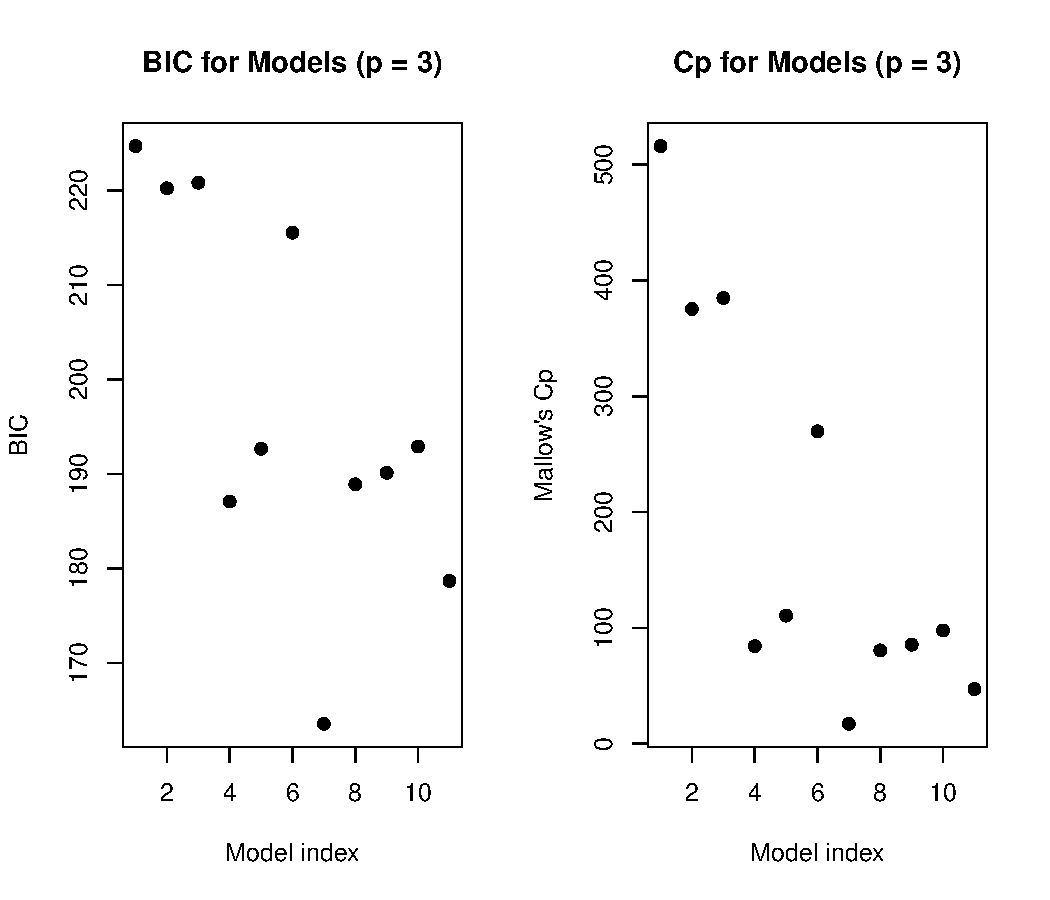
\includegraphics[keepaspectratio]{RMD_files/figure-latex/unnamed-chunk-2-1.pdf}}

\begin{verbatim}
#> integer(0)
\end{verbatim}

\subsection{Part 6}\label{part-6}

Valdation: One of the validation techniques is to compare the SSEp and P
RESSp of the models under considerations. Ideally, these two values
should be close for the same model. Let us use model 11 as an example.
First, we fit this model using lm(), and obtain the SSEp and P RESSp
statistics. The SSEp can be computed based on the component sigma in the
output of summary function. And the P RESSp statistic of a model can be
computed using function press() in the DAAG package. Make sure to
install the package before you run the commands.

\begin{Shaded}
\begin{Highlighting}[]
\CommentTok{\#{-}{-}{-}{-}{-}{-}{-}{-}{-}{-}{-}{-}{-}{-}{-}{-}{-}{-}{-}{-}{-}{-}{-}{-}{-}{-}{-}{-}{-}{-}{-}{-}{-}{-}{-}{-}{-}{-}{-}{-}{-}{-}{-}{-}{-}{-}{-}}
\CommentTok{\# 1) Chuẩn bị dữ liệu và gói cần thiết}
\CommentTok{\#{-}{-}{-}{-}{-}{-}{-}{-}{-}{-}{-}{-}{-}{-}{-}{-}{-}{-}{-}{-}{-}{-}{-}{-}{-}{-}{-}{-}{-}{-}{-}{-}{-}{-}{-}{-}{-}{-}{-}{-}{-}{-}{-}{-}{-}{-}{-}}
\CommentTok{\# install.packages("DAAG") \# cài nếu chưa có}
\FunctionTok{library}\NormalTok{(DAAG)}
\CommentTok{\# install.packages("readxl") \# cài nếu cần đọc Excel}
\FunctionTok{library}\NormalTok{(readxl)}

\CommentTok{\# Giả sử bạn đã đọc dữ liệu vào jobs\_data:}
\NormalTok{jobs\_data }\OtherTok{\textless{}{-}} \FunctionTok{read\_excel}\NormalTok{(}\StringTok{"data.xlsx"}\NormalTok{, }\AttributeTok{col\_names =} \ConstantTok{FALSE}\NormalTok{)}
\CommentTok{\#\textgreater{} New names:}
\CommentTok{\#\textgreater{} * \textasciigrave{}\textasciigrave{} {-}\textgreater{} \textasciigrave{}...1\textasciigrave{}}
\CommentTok{\#\textgreater{} * \textasciigrave{}\textasciigrave{} {-}\textgreater{} \textasciigrave{}...2\textasciigrave{}}
\CommentTok{\#\textgreater{} * \textasciigrave{}\textasciigrave{} {-}\textgreater{} \textasciigrave{}...3\textasciigrave{}}
\CommentTok{\#\textgreater{} * \textasciigrave{}\textasciigrave{} {-}\textgreater{} \textasciigrave{}...4\textasciigrave{}}
\CommentTok{\#\textgreater{} * \textasciigrave{}\textasciigrave{} {-}\textgreater{} \textasciigrave{}...5\textasciigrave{}}
\FunctionTok{colnames}\NormalTok{(jobs\_data) }\OtherTok{\textless{}{-}} \FunctionTok{c}\NormalTok{(}\StringTok{"y"}\NormalTok{, }\StringTok{"t1"}\NormalTok{, }\StringTok{"t2"}\NormalTok{, }\StringTok{"t3"}\NormalTok{, }\StringTok{"t4"}\NormalTok{)}

\CommentTok{\#{-}{-}{-}{-}{-}{-}{-}{-}{-}{-}{-}{-}{-}{-}{-}{-}{-}{-}{-}{-}{-}{-}{-}{-}{-}{-}{-}{-}{-}{-}{-}{-}{-}{-}{-}{-}{-}{-}{-}{-}{-}{-}{-}{-}{-}{-}{-}}
\CommentTok{\# 2) Tạo danh sách tất cả các tổ hợp biến}
\CommentTok{\#{-}{-}{-}{-}{-}{-}{-}{-}{-}{-}{-}{-}{-}{-}{-}{-}{-}{-}{-}{-}{-}{-}{-}{-}{-}{-}{-}{-}{-}{-}{-}{-}{-}{-}{-}{-}{-}{-}{-}{-}{-}{-}{-}{-}{-}{-}{-}}
\NormalTok{predictors }\OtherTok{\textless{}{-}} \FunctionTok{c}\NormalTok{(}\StringTok{"t1"}\NormalTok{, }\StringTok{"t2"}\NormalTok{, }\StringTok{"t3"}\NormalTok{, }\StringTok{"t4"}\NormalTok{)}

\CommentTok{\# Hàm combn() sẽ lấy tất cả tổ hợp k phần tử từ danh sách, }
\CommentTok{\# lapply(...) để duyệt k = 1..4, rồi unlist(..., recursive=FALSE) gộp lại thành một list.}
\NormalTok{subset\_list }\OtherTok{\textless{}{-}} \FunctionTok{unlist}\NormalTok{(}
  \FunctionTok{lapply}\NormalTok{(}\DecValTok{1}\SpecialCharTok{:}\FunctionTok{length}\NormalTok{(predictors), }\ControlFlowTok{function}\NormalTok{(k) \{}
    \FunctionTok{combn}\NormalTok{(predictors, k, }\AttributeTok{simplify =} \ConstantTok{FALSE}\NormalTok{)}
\NormalTok{  \}),}
  \AttributeTok{recursive =} \ConstantTok{FALSE}
\NormalTok{)}

\CommentTok{\#{-}{-}{-}{-}{-}{-}{-}{-}{-}{-}{-}{-}{-}{-}{-}{-}{-}{-}{-}{-}{-}{-}{-}{-}{-}{-}{-}{-}{-}{-}{-}{-}{-}{-}{-}{-}{-}{-}{-}{-}{-}{-}{-}{-}{-}{-}{-}}
\CommentTok{\# 3) Khởi tạo khung kết quả}
\CommentTok{\#{-}{-}{-}{-}{-}{-}{-}{-}{-}{-}{-}{-}{-}{-}{-}{-}{-}{-}{-}{-}{-}{-}{-}{-}{-}{-}{-}{-}{-}{-}{-}{-}{-}{-}{-}{-}{-}{-}{-}{-}{-}{-}{-}{-}{-}{-}{-}}
\NormalTok{results }\OtherTok{\textless{}{-}} \FunctionTok{data.frame}\NormalTok{(}
  \AttributeTok{model =} \FunctionTok{character}\NormalTok{(),}
  \AttributeTok{SSE   =} \FunctionTok{numeric}\NormalTok{(),}
  \AttributeTok{PRESS =} \FunctionTok{numeric}\NormalTok{(),}
  \AttributeTok{stringsAsFactors =} \ConstantTok{FALSE}
\NormalTok{)}

\CommentTok{\# Số dòng (số quan sát)}
\NormalTok{n }\OtherTok{\textless{}{-}} \FunctionTok{nrow}\NormalTok{(jobs\_data)}

\CommentTok{\#{-}{-}{-}{-}{-}{-}{-}{-}{-}{-}{-}{-}{-}{-}{-}{-}{-}{-}{-}{-}{-}{-}{-}{-}{-}{-}{-}{-}{-}{-}{-}{-}{-}{-}{-}{-}{-}{-}{-}{-}{-}{-}{-}{-}{-}{-}{-}}
\CommentTok{\# 4) Vòng lặp: ước lượng từng mô hình, tính SSE \& PRESS}
\CommentTok{\#{-}{-}{-}{-}{-}{-}{-}{-}{-}{-}{-}{-}{-}{-}{-}{-}{-}{-}{-}{-}{-}{-}{-}{-}{-}{-}{-}{-}{-}{-}{-}{-}{-}{-}{-}{-}{-}{-}{-}{-}{-}{-}{-}{-}{-}{-}{-}}
\ControlFlowTok{for}\NormalTok{ (vars }\ControlFlowTok{in}\NormalTok{ subset\_list) \{}
  \CommentTok{\# Tạo chuỗi công thức, ví dụ "y \textasciitilde{} t1 + t3" v.v.}
\NormalTok{  formula\_str }\OtherTok{\textless{}{-}} \FunctionTok{paste}\NormalTok{(}\StringTok{"y \textasciitilde{}"}\NormalTok{, }\FunctionTok{paste}\NormalTok{(vars, }\AttributeTok{collapse =} \StringTok{" + "}\NormalTok{))}
  
  \CommentTok{\# Fit mô hình}
\NormalTok{  fit }\OtherTok{\textless{}{-}} \FunctionTok{lm}\NormalTok{(}\FunctionTok{as.formula}\NormalTok{(formula\_str), }\AttributeTok{data =}\NormalTok{ jobs\_data)}
  
  \CommentTok{\# Tính SSE:}
  \CommentTok{\# {-} Cách 1: Dùng công thức SSE = sigma\^{}2 * (n {-} p),}
  \CommentTok{\#           trong đó p = số tham số (kể cả intercept).}
\NormalTok{  p }\OtherTok{\textless{}{-}} \FunctionTok{length}\NormalTok{(}\FunctionTok{coef}\NormalTok{(fit))               }\CommentTok{\# số tham số ước lượng}
\NormalTok{  rse }\OtherTok{\textless{}{-}} \FunctionTok{summary}\NormalTok{(fit)}\SpecialCharTok{$}\NormalTok{sigma            }\CommentTok{\# residual standard error}
\NormalTok{  SSEp }\OtherTok{\textless{}{-}}\NormalTok{ rse}\SpecialCharTok{\^{}}\DecValTok{2} \SpecialCharTok{*}\NormalTok{ (n }\SpecialCharTok{{-}}\NormalTok{ p)}
  
  \CommentTok{\# {-} Cách 2 (tương đương): SSEp = sum(resid(fit)\^{}2)}
  \CommentTok{\# SSEp \textless{}{-} sum(resid(fit)\^{}2)}

  \CommentTok{\# Tính PRESS:}
\NormalTok{  PRESSp }\OtherTok{\textless{}{-}} \FunctionTok{press}\NormalTok{(fit)  }\CommentTok{\# từ gói DAAG}

  \CommentTok{\# Lưu kết quả}
\NormalTok{  results }\OtherTok{\textless{}{-}} \FunctionTok{rbind}\NormalTok{(results, }\FunctionTok{data.frame}\NormalTok{(}
    \AttributeTok{model =}\NormalTok{ formula\_str,}
    \AttributeTok{SSE   =}\NormalTok{ SSEp,}
    \AttributeTok{PRESS =}\NormalTok{ PRESSp}
\NormalTok{  ))}
\NormalTok{\}}

\CommentTok{\#{-}{-}{-}{-}{-}{-}{-}{-}{-}{-}{-}{-}{-}{-}{-}{-}{-}{-}{-}{-}{-}{-}{-}{-}{-}{-}{-}{-}{-}{-}{-}{-}{-}{-}{-}{-}{-}{-}{-}{-}{-}{-}{-}{-}{-}{-}{-}}
\CommentTok{\# 5) Xem kết quả}
\CommentTok{\#{-}{-}{-}{-}{-}{-}{-}{-}{-}{-}{-}{-}{-}{-}{-}{-}{-}{-}{-}{-}{-}{-}{-}{-}{-}{-}{-}{-}{-}{-}{-}{-}{-}{-}{-}{-}{-}{-}{-}{-}{-}{-}{-}{-}{-}{-}{-}}
\NormalTok{knitr}\SpecialCharTok{::}\FunctionTok{kable}\NormalTok{(results, }\AttributeTok{caption =} \StringTok{"Bảng kết quả"}\NormalTok{)}
\end{Highlighting}
\end{Shaded}

\begin{longtable}[]{@{}lrr@{}}
\caption{Bảng kết quả}\tabularnewline
\toprule\noalign{}
model & SSE & PRESS \\
\midrule\noalign{}
\endfirsthead
\toprule\noalign{}
model & SSE & PRESS \\
\midrule\noalign{}
\endhead
\bottomrule\noalign{}
\endlastfoot
y \textasciitilde{} t1 & 6658.1453 & 7791.5994 \\
y \textasciitilde{} t2 & 6817.5291 & 7991.0964 \\
y \textasciitilde{} t3 & 1768.0228 & 2064.5976 \\
y \textasciitilde{} t4 & 2210.6887 & 2548.6349 \\
y \textasciitilde{} t1 + t2 & 4851.1799 & 6444.0411 \\
y \textasciitilde{} t1 + t3 & 606.6574 & 760.9744 \\
y \textasciitilde{} t1 + t4 & 1672.5853 & 2109.8967 \\
y \textasciitilde{} t2 + t3 & 1755.8127 & 2206.6460 \\
y \textasciitilde{} t2 + t4 & 1962.0716 & 2491.7979 \\
y \textasciitilde{} t3 + t4 & 1111.3126 & 1449.6001 \\
y \textasciitilde{} t1 + t2 + t3 & 596.7207 & 831.1521 \\
y \textasciitilde{} t1 + t2 + t4 & 1400.1275 & 1885.8454 \\
y \textasciitilde{} t1 + t3 + t4 & 348.1970 & 471.4520 \\
y \textasciitilde{} t2 + t3 + t4 & 1095.8078 & 1570.5610 \\
y \textasciitilde{} t1 + t2 + t3 + t4 & 335.9775 & 518.9885 \\
\end{longtable}

\subsection{Part 7}\label{part-7}

Automated search procedure: Next we explore forward selection, backward
elimination, and stepwise regression. These are performed using the
step() function. In forward selection, to start from a model with just
the intercept and end with a model with all variables. Do the same with
backward elimination. What model(s) is chosen with these procedures? It
is important to bear in mind that the same model is not always going to
be selected by all of these procedures, and the choice of starting model
might impact the result.

\begin{Shaded}
\begin{Highlighting}[]
\FunctionTok{library}\NormalTok{(readxl)}
\FunctionTok{library}\NormalTok{(ggplot2)}
\FunctionTok{library}\NormalTok{(MASS)}

\CommentTok{\# Đọc dữ liệu}
\NormalTok{jobs\_data }\OtherTok{\textless{}{-}} \FunctionTok{read\_excel}\NormalTok{(}\StringTok{"data.xlsx"}\NormalTok{, }\AttributeTok{col\_names =} \ConstantTok{FALSE}\NormalTok{)}
\CommentTok{\#\textgreater{} New names:}
\CommentTok{\#\textgreater{} * \textasciigrave{}\textasciigrave{} {-}\textgreater{} \textasciigrave{}...1\textasciigrave{}}
\CommentTok{\#\textgreater{} * \textasciigrave{}\textasciigrave{} {-}\textgreater{} \textasciigrave{}...2\textasciigrave{}}
\CommentTok{\#\textgreater{} * \textasciigrave{}\textasciigrave{} {-}\textgreater{} \textasciigrave{}...3\textasciigrave{}}
\CommentTok{\#\textgreater{} * \textasciigrave{}\textasciigrave{} {-}\textgreater{} \textasciigrave{}...4\textasciigrave{}}
\CommentTok{\#\textgreater{} * \textasciigrave{}\textasciigrave{} {-}\textgreater{} \textasciigrave{}...5\textasciigrave{}}
\FunctionTok{colnames}\NormalTok{(jobs\_data) }\OtherTok{\textless{}{-}} \FunctionTok{c}\NormalTok{(}\StringTok{"y"}\NormalTok{, }\StringTok{"t1"}\NormalTok{, }\StringTok{"t2"}\NormalTok{, }\StringTok{"t3"}\NormalTok{, }\StringTok{"t4"}\NormalTok{)}

\CommentTok{\# Mô hình null (chỉ có intercept) và mô hình đầy đủ}
\NormalTok{null\_model }\OtherTok{\textless{}{-}} \FunctionTok{lm}\NormalTok{(y }\SpecialCharTok{\textasciitilde{}} \DecValTok{1}\NormalTok{, }\AttributeTok{data =}\NormalTok{ jobs\_data)}
\NormalTok{full\_model }\OtherTok{\textless{}{-}} \FunctionTok{lm}\NormalTok{(y }\SpecialCharTok{\textasciitilde{}}\NormalTok{ t1 }\SpecialCharTok{+}\NormalTok{ t2 }\SpecialCharTok{+}\NormalTok{ t3 }\SpecialCharTok{+}\NormalTok{ t4, }\AttributeTok{data =}\NormalTok{ jobs\_data)}

\CommentTok{\# Forward Selection}
\NormalTok{forward\_model }\OtherTok{\textless{}{-}} \FunctionTok{step}\NormalTok{(null\_model, }\AttributeTok{scope =} \FunctionTok{list}\NormalTok{(}\AttributeTok{lower =}\NormalTok{ null\_model, }\AttributeTok{upper =}\NormalTok{ full\_model), }\AttributeTok{direction =} \StringTok{"forward"}\NormalTok{)}
\CommentTok{\#\textgreater{} Start:  AIC=149.3}
\CommentTok{\#\textgreater{} y \textasciitilde{} 1}
\CommentTok{\#\textgreater{} }
\CommentTok{\#\textgreater{}        Df Sum of Sq    RSS    AIC}
\CommentTok{\#\textgreater{} + t3    1    7286.0 1768.0 110.47}
\CommentTok{\#\textgreater{} + t4    1    6843.3 2210.7 116.06}
\CommentTok{\#\textgreater{} + t1    1    2395.9 6658.1 143.62}
\CommentTok{\#\textgreater{} + t2    1    2236.5 6817.5 144.21}
\CommentTok{\#\textgreater{} \textless{}none\textgreater{}              9054.0 149.30}
\CommentTok{\#\textgreater{} }
\CommentTok{\#\textgreater{} Step:  AIC=110.47}
\CommentTok{\#\textgreater{} y \textasciitilde{} t3}
\CommentTok{\#\textgreater{} }
\CommentTok{\#\textgreater{}        Df Sum of Sq     RSS     AIC}
\CommentTok{\#\textgreater{} + t1    1   1161.37  606.66  85.727}
\CommentTok{\#\textgreater{} + t4    1    656.71 1111.31 100.861}
\CommentTok{\#\textgreater{} \textless{}none\textgreater{}              1768.02 110.469}
\CommentTok{\#\textgreater{} + t2    1     12.21 1755.81 112.295}
\CommentTok{\#\textgreater{} }
\CommentTok{\#\textgreater{} Step:  AIC=85.73}
\CommentTok{\#\textgreater{} y \textasciitilde{} t3 + t1}
\CommentTok{\#\textgreater{} }
\CommentTok{\#\textgreater{}        Df Sum of Sq    RSS    AIC}
\CommentTok{\#\textgreater{} + t4    1   258.460 348.20 73.847}
\CommentTok{\#\textgreater{} \textless{}none\textgreater{}              606.66 85.727}
\CommentTok{\#\textgreater{} + t2    1     9.937 596.72 87.314}
\CommentTok{\#\textgreater{} }
\CommentTok{\#\textgreater{} Step:  AIC=73.85}
\CommentTok{\#\textgreater{} y \textasciitilde{} t3 + t1 + t4}
\CommentTok{\#\textgreater{} }
\CommentTok{\#\textgreater{}        Df Sum of Sq    RSS    AIC}
\CommentTok{\#\textgreater{} \textless{}none\textgreater{}              348.20 73.847}
\CommentTok{\#\textgreater{} + t2    1     12.22 335.98 74.954}

\CommentTok{\# Backward Elimination}
\NormalTok{backward\_model }\OtherTok{\textless{}{-}} \FunctionTok{step}\NormalTok{(full\_model, }\AttributeTok{direction =} \StringTok{"backward"}\NormalTok{)}
\CommentTok{\#\textgreater{} Start:  AIC=74.95}
\CommentTok{\#\textgreater{} y \textasciitilde{} t1 + t2 + t3 + t4}
\CommentTok{\#\textgreater{} }
\CommentTok{\#\textgreater{}        Df Sum of Sq     RSS     AIC}
\CommentTok{\#\textgreater{} {-} t2    1     12.22  348.20  73.847}
\CommentTok{\#\textgreater{} \textless{}none\textgreater{}               335.98  74.954}
\CommentTok{\#\textgreater{} {-} t4    1    260.74  596.72  87.314}
\CommentTok{\#\textgreater{} {-} t1    1    759.83 1095.81 102.509}
\CommentTok{\#\textgreater{} {-} t3    1   1064.15 1400.13 108.636}
\CommentTok{\#\textgreater{} }
\CommentTok{\#\textgreater{} Step:  AIC=73.85}
\CommentTok{\#\textgreater{} y \textasciitilde{} t1 + t3 + t4}
\CommentTok{\#\textgreater{} }
\CommentTok{\#\textgreater{}        Df Sum of Sq     RSS     AIC}
\CommentTok{\#\textgreater{} \textless{}none\textgreater{}               348.20  73.847}
\CommentTok{\#\textgreater{} {-} t4    1    258.46  606.66  85.727}
\CommentTok{\#\textgreater{} {-} t1    1    763.12 1111.31 100.861}
\CommentTok{\#\textgreater{} {-} t3    1   1324.39 1672.59 111.081}

\CommentTok{\# Stepwise Regression}
\NormalTok{stepwise\_model }\OtherTok{\textless{}{-}} \FunctionTok{step}\NormalTok{(null\_model, }\AttributeTok{scope =} \FunctionTok{list}\NormalTok{(}\AttributeTok{lower =}\NormalTok{ null\_model, }\AttributeTok{upper =}\NormalTok{ full\_model), }\AttributeTok{direction =} \StringTok{"both"}\NormalTok{)}
\CommentTok{\#\textgreater{} Start:  AIC=149.3}
\CommentTok{\#\textgreater{} y \textasciitilde{} 1}
\CommentTok{\#\textgreater{} }
\CommentTok{\#\textgreater{}        Df Sum of Sq    RSS    AIC}
\CommentTok{\#\textgreater{} + t3    1    7286.0 1768.0 110.47}
\CommentTok{\#\textgreater{} + t4    1    6843.3 2210.7 116.06}
\CommentTok{\#\textgreater{} + t1    1    2395.9 6658.1 143.62}
\CommentTok{\#\textgreater{} + t2    1    2236.5 6817.5 144.21}
\CommentTok{\#\textgreater{} \textless{}none\textgreater{}              9054.0 149.30}
\CommentTok{\#\textgreater{} }
\CommentTok{\#\textgreater{} Step:  AIC=110.47}
\CommentTok{\#\textgreater{} y \textasciitilde{} t3}
\CommentTok{\#\textgreater{} }
\CommentTok{\#\textgreater{}        Df Sum of Sq    RSS     AIC}
\CommentTok{\#\textgreater{} + t1    1    1161.4  606.7  85.727}
\CommentTok{\#\textgreater{} + t4    1     656.7 1111.3 100.861}
\CommentTok{\#\textgreater{} \textless{}none\textgreater{}              1768.0 110.469}
\CommentTok{\#\textgreater{} + t2    1      12.2 1755.8 112.295}
\CommentTok{\#\textgreater{} {-} t3    1    7286.0 9054.0 149.302}
\CommentTok{\#\textgreater{} }
\CommentTok{\#\textgreater{} Step:  AIC=85.73}
\CommentTok{\#\textgreater{} y \textasciitilde{} t3 + t1}
\CommentTok{\#\textgreater{} }
\CommentTok{\#\textgreater{}        Df Sum of Sq    RSS     AIC}
\CommentTok{\#\textgreater{} + t4    1     258.5  348.2  73.847}
\CommentTok{\#\textgreater{} \textless{}none\textgreater{}               606.7  85.727}
\CommentTok{\#\textgreater{} + t2    1       9.9  596.7  87.314}
\CommentTok{\#\textgreater{} {-} t1    1    1161.4 1768.0 110.469}
\CommentTok{\#\textgreater{} {-} t3    1    6051.5 6658.1 143.618}
\CommentTok{\#\textgreater{} }
\CommentTok{\#\textgreater{} Step:  AIC=73.85}
\CommentTok{\#\textgreater{} y \textasciitilde{} t3 + t1 + t4}
\CommentTok{\#\textgreater{} }
\CommentTok{\#\textgreater{}        Df Sum of Sq     RSS     AIC}
\CommentTok{\#\textgreater{} \textless{}none\textgreater{}               348.20  73.847}
\CommentTok{\#\textgreater{} + t2    1     12.22  335.98  74.954}
\CommentTok{\#\textgreater{} {-} t4    1    258.46  606.66  85.727}
\CommentTok{\#\textgreater{} {-} t1    1    763.12 1111.31 100.861}
\CommentTok{\#\textgreater{} {-} t3    1   1324.39 1672.59 111.081}

\CommentTok{\# Thêm dự đoán vào dữ liệu}
\NormalTok{jobs\_data}\SpecialCharTok{$}\NormalTok{pred\_forward }\OtherTok{\textless{}{-}} \FunctionTok{predict}\NormalTok{(forward\_model, jobs\_data)}
\NormalTok{jobs\_data}\SpecialCharTok{$}\NormalTok{pred\_backward }\OtherTok{\textless{}{-}} \FunctionTok{predict}\NormalTok{(backward\_model, jobs\_data)}
\NormalTok{jobs\_data}\SpecialCharTok{$}\NormalTok{pred\_stepwise }\OtherTok{\textless{}{-}} \FunctionTok{predict}\NormalTok{(stepwise\_model, jobs\_data)}
\end{Highlighting}
\end{Shaded}

\begin{Shaded}
\begin{Highlighting}[]
\CommentTok{\# Biểu đồ so sánh giá trị thực tế và dự đoán}
\FunctionTok{ggplot}\NormalTok{(jobs\_data, }\FunctionTok{aes}\NormalTok{(}\AttributeTok{x =}\NormalTok{ y)) }\SpecialCharTok{+}
  \FunctionTok{geom\_point}\NormalTok{(}\FunctionTok{aes}\NormalTok{(}\AttributeTok{y =}\NormalTok{ pred\_forward, }\AttributeTok{color =} \StringTok{"Forward Selection"}\NormalTok{)) }\SpecialCharTok{+}
  \FunctionTok{geom\_point}\NormalTok{(}\FunctionTok{aes}\NormalTok{(}\AttributeTok{y =}\NormalTok{ pred\_backward, }\AttributeTok{color =} \StringTok{"Backward Elimination"}\NormalTok{)) }\SpecialCharTok{+}
  \FunctionTok{geom\_point}\NormalTok{(}\FunctionTok{aes}\NormalTok{(}\AttributeTok{y =}\NormalTok{ pred\_stepwise, }\AttributeTok{color =} \StringTok{"Stepwise Regression"}\NormalTok{)) }\SpecialCharTok{+}
  \FunctionTok{geom\_abline}\NormalTok{(}\AttributeTok{slope =} \DecValTok{1}\NormalTok{, }\AttributeTok{intercept =} \DecValTok{0}\NormalTok{, }\AttributeTok{linetype =} \StringTok{"dashed"}\NormalTok{) }\SpecialCharTok{+} 
  \FunctionTok{labs}\NormalTok{(}\AttributeTok{title =} \StringTok{"Actual vs Predicted Values"}\NormalTok{, }\AttributeTok{x =} \StringTok{"Actual y"}\NormalTok{, }\AttributeTok{y =} \StringTok{"Predicted y"}\NormalTok{) }\SpecialCharTok{+}
  \FunctionTok{theme\_minimal}\NormalTok{() }\SpecialCharTok{+}
  \FunctionTok{scale\_color\_manual}\NormalTok{(}\AttributeTok{values =} \FunctionTok{c}\NormalTok{(}\StringTok{"red"}\NormalTok{, }\StringTok{"blue"}\NormalTok{, }\StringTok{"green"}\NormalTok{))}
\end{Highlighting}
\end{Shaded}

\pandocbounded{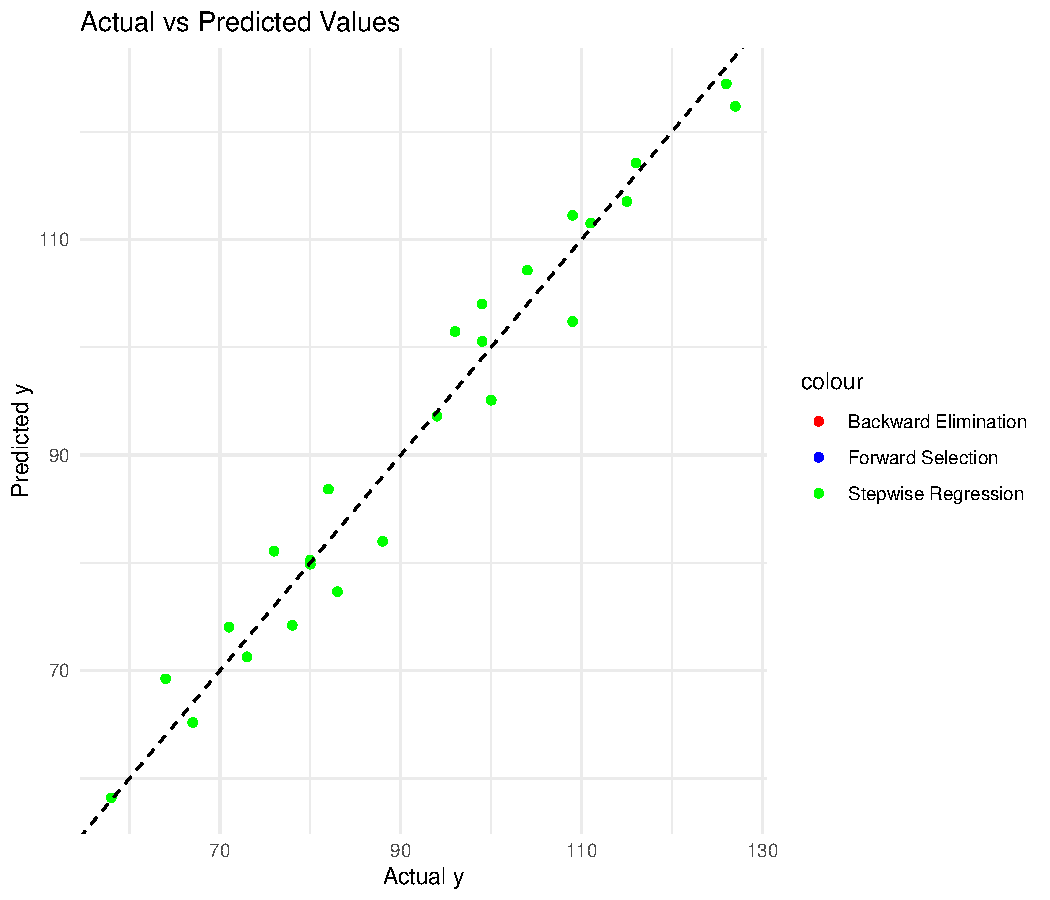
\includegraphics[keepaspectratio]{RMD_files/figure-latex/unnamed-chunk-5-1.pdf}}

\begin{Shaded}
\begin{Highlighting}[]
\CommentTok{\# Biểu đồ Residuals để kiểm tra mô hình}
\FunctionTok{ggplot}\NormalTok{(jobs\_data, }\FunctionTok{aes}\NormalTok{(}\AttributeTok{x =}\NormalTok{ pred\_forward, }\AttributeTok{y =} \FunctionTok{residuals}\NormalTok{(forward\_model))) }\SpecialCharTok{+}
  \FunctionTok{geom\_point}\NormalTok{(}\AttributeTok{color =} \StringTok{"red"}\NormalTok{) }\SpecialCharTok{+}
  \FunctionTok{geom\_hline}\NormalTok{(}\AttributeTok{yintercept =} \DecValTok{0}\NormalTok{, }\AttributeTok{linetype =} \StringTok{"dashed"}\NormalTok{) }\SpecialCharTok{+}
  \FunctionTok{labs}\NormalTok{(}\AttributeTok{title =} \StringTok{"Residual Plot {-} Forward Selection"}\NormalTok{, }\AttributeTok{x =} \StringTok{"Predicted Values"}\NormalTok{, }\AttributeTok{y =} \StringTok{"Residuals"}\NormalTok{) }\SpecialCharTok{+}
  \FunctionTok{theme\_minimal}\NormalTok{()}
\end{Highlighting}
\end{Shaded}

\pandocbounded{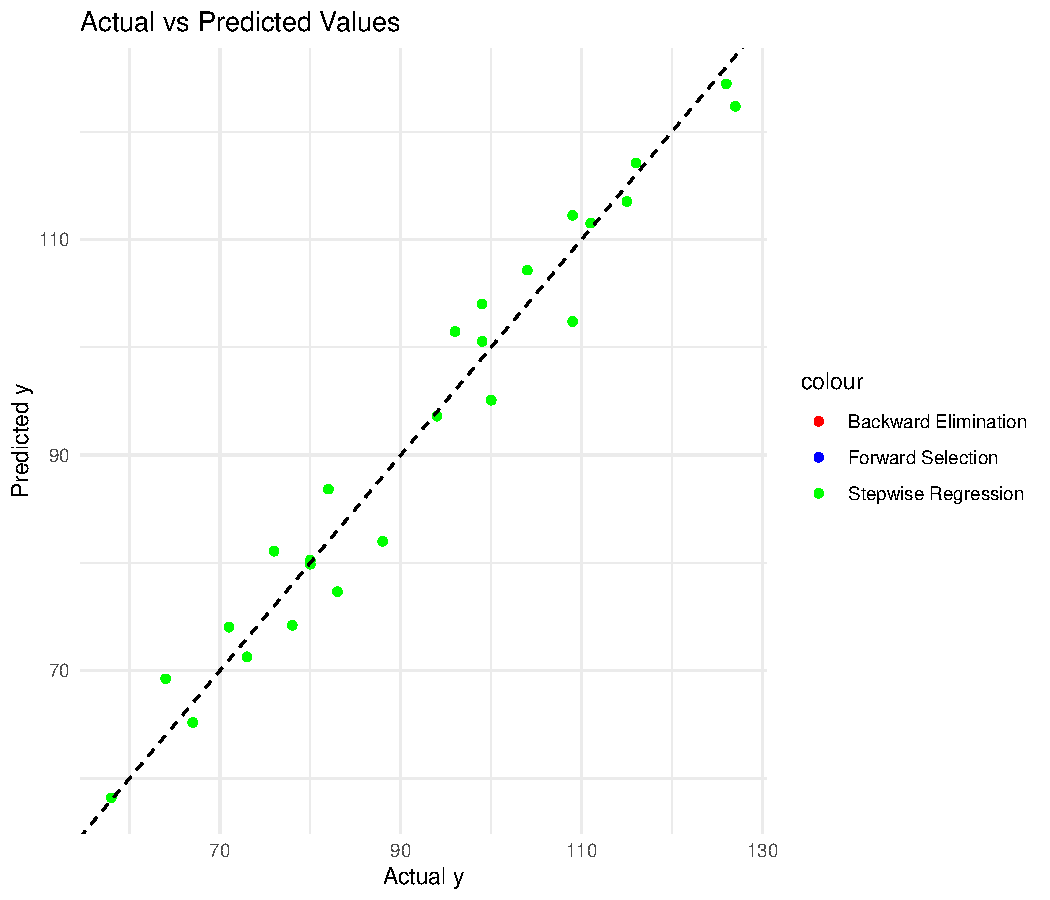
\includegraphics[keepaspectratio]{RMD_files/figure-latex/unnamed-chunk-6-1.pdf}}

\section{So sánh AIC của các mô
hình}\label{so-suxe1nh-aic-cux1ee7a-cuxe1c-muxf4-huxecnh}

aic\_values \textless- data.frame( Model = c(``Forward Selection'',
``Backward Elimination'', ``Stepwise Regression''), AIC =
c(AIC(forward\_model), AIC(backward\_model), AIC(stepwise\_model)) )

\begin{Shaded}
\begin{Highlighting}[]
\FunctionTok{ggplot}\NormalTok{(aic\_values, }\FunctionTok{aes}\NormalTok{(}\AttributeTok{x =}\NormalTok{ Model, }\AttributeTok{y =}\NormalTok{ AIC, }\AttributeTok{fill =}\NormalTok{ Model)) }\SpecialCharTok{+}
  \FunctionTok{geom\_bar}\NormalTok{(}\AttributeTok{stat =} \StringTok{"identity"}\NormalTok{, }\AttributeTok{width =} \FloatTok{0.5}\NormalTok{) }\SpecialCharTok{+}
  \FunctionTok{labs}\NormalTok{(}\AttributeTok{title =} \StringTok{"AIC Comparison of Models"}\NormalTok{, }\AttributeTok{y =} \StringTok{"AIC Value"}\NormalTok{) }\SpecialCharTok{+}
  \FunctionTok{theme\_minimal}\NormalTok{() }\SpecialCharTok{+}
  \FunctionTok{scale\_fill\_manual}\NormalTok{(}\AttributeTok{values =} \FunctionTok{c}\NormalTok{(}\StringTok{"red"}\NormalTok{, }\StringTok{"blue"}\NormalTok{, }\StringTok{"green"}\NormalTok{))}
\end{Highlighting}
\end{Shaded}

\pandocbounded{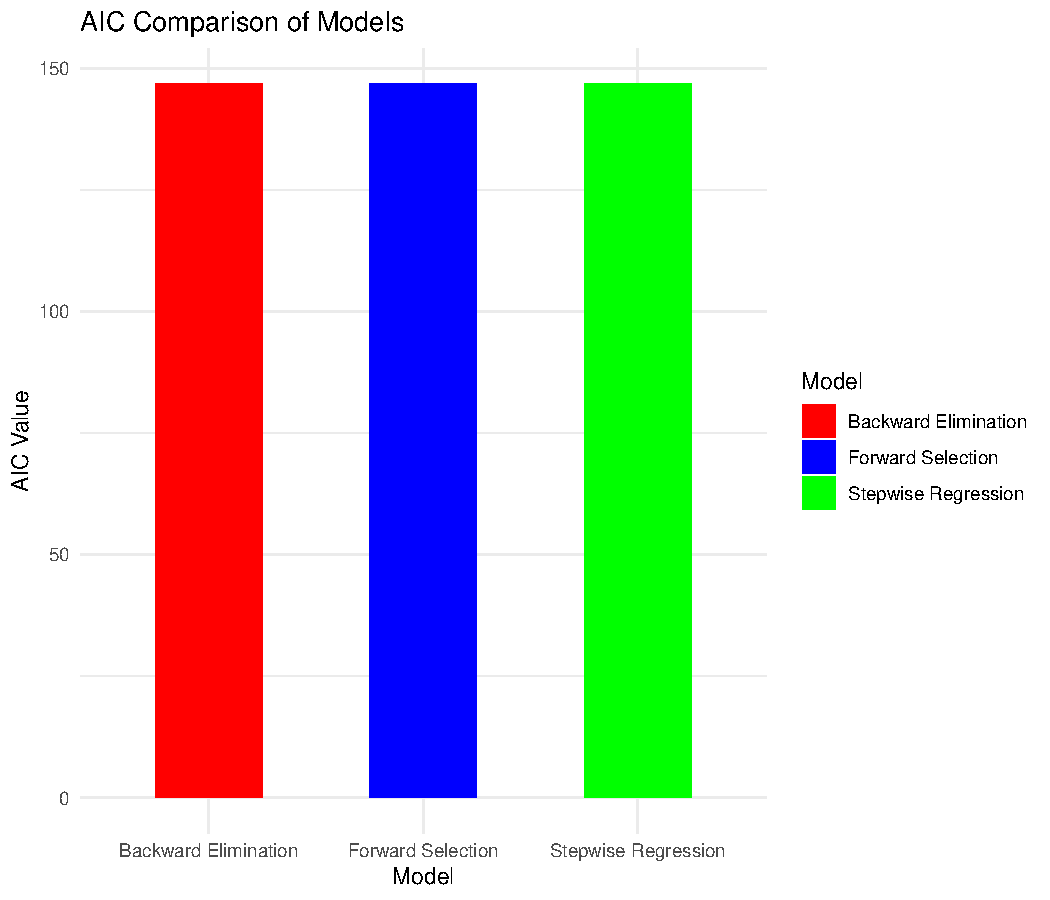
\includegraphics[keepaspectratio]{RMD_files/figure-latex/unnamed-chunk-7-1.pdf}}

\begin{Shaded}
\begin{Highlighting}[]
  \CommentTok{\# In summary các mô hình}
\FunctionTok{cat}\NormalTok{(}\StringTok{"Forward Selection Model Summary:}\SpecialCharTok{\textbackslash{}n}\StringTok{"}\NormalTok{)}
\CommentTok{\#\textgreater{} Forward Selection Model Summary:}
\FunctionTok{print}\NormalTok{(}\FunctionTok{summary}\NormalTok{(forward\_model))}
\CommentTok{\#\textgreater{} }
\CommentTok{\#\textgreater{} Call:}
\CommentTok{\#\textgreater{} lm(formula = y \textasciitilde{} t3 + t1 + t4, data = jobs\_data)}
\CommentTok{\#\textgreater{} }
\CommentTok{\#\textgreater{} Residuals:}
\CommentTok{\#\textgreater{}     Min      1Q  Median      3Q     Max }
\CommentTok{\#\textgreater{} {-}5.4579 {-}3.1563 {-}0.2057  1.8070  6.6083 }
\CommentTok{\#\textgreater{} }
\CommentTok{\#\textgreater{} Coefficients:}
\CommentTok{\#\textgreater{}               Estimate Std. Error t value Pr(\textgreater{}|t|)    }
\CommentTok{\#\textgreater{} (Intercept) {-}124.20002    9.87406 {-}12.578 3.04e{-}11 ***}
\CommentTok{\#\textgreater{} t3             1.35697    0.15183   8.937 1.33e{-}08 ***}
\CommentTok{\#\textgreater{} t1             0.29633    0.04368   6.784 1.04e{-}06 ***}
\CommentTok{\#\textgreater{} t4             0.51742    0.13105   3.948 0.000735 ***}
\CommentTok{\#\textgreater{} {-}{-}{-}}
\CommentTok{\#\textgreater{} Signif. codes:  0 \textquotesingle{}***\textquotesingle{} 0.001 \textquotesingle{}**\textquotesingle{} 0.01 \textquotesingle{}*\textquotesingle{} 0.05 \textquotesingle{}.\textquotesingle{} 0.1 \textquotesingle{} \textquotesingle{} 1}
\CommentTok{\#\textgreater{} }
\CommentTok{\#\textgreater{} Residual standard error: 4.072 on 21 degrees of freedom}
\CommentTok{\#\textgreater{} Multiple R{-}squared:  0.9615, Adjusted R{-}squared:  0.956 }
\CommentTok{\#\textgreater{} F{-}statistic:   175 on 3 and 21 DF,  p{-}value: 5.16e{-}15}

\FunctionTok{cat}\NormalTok{(}\StringTok{"}\SpecialCharTok{\textbackslash{}n}\StringTok{Backward Elimination Model Summary:}\SpecialCharTok{\textbackslash{}n}\StringTok{"}\NormalTok{)}
\CommentTok{\#\textgreater{} }
\CommentTok{\#\textgreater{} Backward Elimination Model Summary:}
\FunctionTok{print}\NormalTok{(}\FunctionTok{summary}\NormalTok{(backward\_model))}
\CommentTok{\#\textgreater{} }
\CommentTok{\#\textgreater{} Call:}
\CommentTok{\#\textgreater{} lm(formula = y \textasciitilde{} t1 + t3 + t4, data = jobs\_data)}
\CommentTok{\#\textgreater{} }
\CommentTok{\#\textgreater{} Residuals:}
\CommentTok{\#\textgreater{}     Min      1Q  Median      3Q     Max }
\CommentTok{\#\textgreater{} {-}5.4579 {-}3.1563 {-}0.2057  1.8070  6.6083 }
\CommentTok{\#\textgreater{} }
\CommentTok{\#\textgreater{} Coefficients:}
\CommentTok{\#\textgreater{}               Estimate Std. Error t value Pr(\textgreater{}|t|)    }
\CommentTok{\#\textgreater{} (Intercept) {-}124.20002    9.87406 {-}12.578 3.04e{-}11 ***}
\CommentTok{\#\textgreater{} t1             0.29633    0.04368   6.784 1.04e{-}06 ***}
\CommentTok{\#\textgreater{} t3             1.35697    0.15183   8.937 1.33e{-}08 ***}
\CommentTok{\#\textgreater{} t4             0.51742    0.13105   3.948 0.000735 ***}
\CommentTok{\#\textgreater{} {-}{-}{-}}
\CommentTok{\#\textgreater{} Signif. codes:  0 \textquotesingle{}***\textquotesingle{} 0.001 \textquotesingle{}**\textquotesingle{} 0.01 \textquotesingle{}*\textquotesingle{} 0.05 \textquotesingle{}.\textquotesingle{} 0.1 \textquotesingle{} \textquotesingle{} 1}
\CommentTok{\#\textgreater{} }
\CommentTok{\#\textgreater{} Residual standard error: 4.072 on 21 degrees of freedom}
\CommentTok{\#\textgreater{} Multiple R{-}squared:  0.9615, Adjusted R{-}squared:  0.956 }
\CommentTok{\#\textgreater{} F{-}statistic:   175 on 3 and 21 DF,  p{-}value: 5.16e{-}15}

\FunctionTok{cat}\NormalTok{(}\StringTok{"}\SpecialCharTok{\textbackslash{}n}\StringTok{Stepwise Regression Model Summary:}\SpecialCharTok{\textbackslash{}n}\StringTok{"}\NormalTok{)}
\CommentTok{\#\textgreater{} }
\CommentTok{\#\textgreater{} Stepwise Regression Model Summary:}
\FunctionTok{print}\NormalTok{(}\FunctionTok{summary}\NormalTok{(stepwise\_model))}
\CommentTok{\#\textgreater{} }
\CommentTok{\#\textgreater{} Call:}
\CommentTok{\#\textgreater{} lm(formula = y \textasciitilde{} t3 + t1 + t4, data = jobs\_data)}
\CommentTok{\#\textgreater{} }
\CommentTok{\#\textgreater{} Residuals:}
\CommentTok{\#\textgreater{}     Min      1Q  Median      3Q     Max }
\CommentTok{\#\textgreater{} {-}5.4579 {-}3.1563 {-}0.2057  1.8070  6.6083 }
\CommentTok{\#\textgreater{} }
\CommentTok{\#\textgreater{} Coefficients:}
\CommentTok{\#\textgreater{}               Estimate Std. Error t value Pr(\textgreater{}|t|)    }
\CommentTok{\#\textgreater{} (Intercept) {-}124.20002    9.87406 {-}12.578 3.04e{-}11 ***}
\CommentTok{\#\textgreater{} t3             1.35697    0.15183   8.937 1.33e{-}08 ***}
\CommentTok{\#\textgreater{} t1             0.29633    0.04368   6.784 1.04e{-}06 ***}
\CommentTok{\#\textgreater{} t4             0.51742    0.13105   3.948 0.000735 ***}
\CommentTok{\#\textgreater{} {-}{-}{-}}
\CommentTok{\#\textgreater{} Signif. codes:  0 \textquotesingle{}***\textquotesingle{} 0.001 \textquotesingle{}**\textquotesingle{} 0.01 \textquotesingle{}*\textquotesingle{} 0.05 \textquotesingle{}.\textquotesingle{} 0.1 \textquotesingle{} \textquotesingle{} 1}
\CommentTok{\#\textgreater{} }
\CommentTok{\#\textgreater{} Residual standard error: 4.072 on 21 degrees of freedom}
\CommentTok{\#\textgreater{} Multiple R{-}squared:  0.9615, Adjusted R{-}squared:  0.956 }
\CommentTok{\#\textgreater{} F{-}statistic:   175 on 3 and 21 DF,  p{-}value: 5.16e{-}15}

\CommentTok{\# In bảng AIC}
\NormalTok{aic\_values }\OtherTok{\textless{}{-}} \FunctionTok{data.frame}\NormalTok{(}
  \AttributeTok{Model =} \FunctionTok{c}\NormalTok{(}\StringTok{"Forward Selection"}\NormalTok{, }\StringTok{"Backward Elimination"}\NormalTok{, }\StringTok{"Stepwise Regression"}\NormalTok{),}
  \AttributeTok{AIC =} \FunctionTok{c}\NormalTok{(}\FunctionTok{AIC}\NormalTok{(forward\_model), }\FunctionTok{AIC}\NormalTok{(backward\_model), }\FunctionTok{AIC}\NormalTok{(stepwise\_model))}
\NormalTok{)}
\NormalTok{knitr}\SpecialCharTok{::}\FunctionTok{kable}\NormalTok{(aic\_values)}
\end{Highlighting}
\end{Shaded}

\begin{longtable}[]{@{}lr@{}}
\toprule\noalign{}
Model & AIC \\
\midrule\noalign{}
\endhead
\bottomrule\noalign{}
\endlastfoot
Forward Selection & 146.7942 \\
Backward Elimination & 146.7942 \\
Stepwise Regression & 146.7942 \\
\end{longtable}

\subsection{Part 8}\label{part-8}

Searching all models based on specified conditions: Here we introduce a
more powerful model searching function: regsubsets() from the leaps
package. This function allows user to specify certain predictors that
must always be considered, certain predictors that must always be
excluded, and the maximum number of predictors to be considered. A
drawback of this function is that it only considers R2 a,p, Mallow's Cp,
BICp. Find the best models in terms of these criteria.

\begin{Shaded}
\begin{Highlighting}[]
\CommentTok{\# install.packages("leaps")   \# nếu chưa cài}
\FunctionTok{library}\NormalTok{(leaps)}
\FunctionTok{library}\NormalTok{(readxl)}
\CommentTok{\# Ví dụ: Dữ liệu có cột: y, t1, t2, t3, t4}
\NormalTok{jobs\_data }\OtherTok{\textless{}{-}} \FunctionTok{read\_excel}\NormalTok{(}\StringTok{"data.xlsx"}\NormalTok{)}
\FunctionTok{colnames}\NormalTok{(jobs\_data) }\OtherTok{\textless{}{-}} \FunctionTok{c}\NormalTok{(}\StringTok{"y"}\NormalTok{, }\StringTok{"t1"}\NormalTok{, }\StringTok{"t2"}\NormalTok{, }\StringTok{"t3"}\NormalTok{, }\StringTok{"t4"}\NormalTok{)}
\CommentTok{\# Tìm mô hình tốt nhất theo mọi số biến (từ 1 đến 4) trong \{t1, t2, t3, t4\}}
\CommentTok{\# nbest=1 nghĩa là chỉ lấy 1 mô hình tốt nhất cho mỗi số biến.}
\NormalTok{fit\_sub }\OtherTok{\textless{}{-}} \FunctionTok{regsubsets}\NormalTok{(y }\SpecialCharTok{\textasciitilde{}}\NormalTok{ t1 }\SpecialCharTok{+}\NormalTok{ t2 }\SpecialCharTok{+}\NormalTok{ t3 }\SpecialCharTok{+}\NormalTok{ t4,}
                      \AttributeTok{data =}\NormalTok{ jobs\_data,}
                      \AttributeTok{method =} \StringTok{"exhaustive"}\NormalTok{,  }\CommentTok{\# duyệt tất cả tổ hợp}
                      \AttributeTok{nbest =} \DecValTok{1}\NormalTok{,}
                      \AttributeTok{nvmax =} \DecValTok{4}\NormalTok{)              }\CommentTok{\# tối đa 4 biến (có thể ít hơn)}
\NormalTok{summary\_sub }\OtherTok{\textless{}{-}} \FunctionTok{summary}\NormalTok{(fit\_sub)}

\CommentTok{\# summary\_sub$which  =\textgreater{} Ma trận TRUE/FALSE cho biết biến nào được chọn}
\CommentTok{\# summary\_sub$rsq    =\textgreater{} R\^{}2}
\CommentTok{\# summary\_sub$adjr2  =\textgreater{} Adjusted R\^{}2}
\CommentTok{\# summary\_sub$cp     =\textgreater{} Mallow\textquotesingle{}s Cp}
\CommentTok{\# summary\_sub$bic    =\textgreater{} BIC}
\CommentTok{\# 1) Mô hình tốt nhất theo Adjusted R\^{}2 (lớn nhất)}
\NormalTok{best\_adjr2\_index }\OtherTok{\textless{}{-}} \FunctionTok{which.max}\NormalTok{(summary\_sub}\SpecialCharTok{$}\NormalTok{adjr2)}

\CommentTok{\# 2) Mô hình tốt nhất theo Mallow\textquotesingle{}s Cp (nhỏ nhất)}
\NormalTok{best\_cp\_index }\OtherTok{\textless{}{-}} \FunctionTok{which.min}\NormalTok{(summary\_sub}\SpecialCharTok{$}\NormalTok{cp)}

\CommentTok{\# 3) Mô hình tốt nhất theo BIC (nhỏ nhất)}
\NormalTok{best\_bic\_index }\OtherTok{\textless{}{-}} \FunctionTok{which.min}\NormalTok{(summary\_sub}\SpecialCharTok{$}\NormalTok{bic)}

\CommentTok{\# Kiểm tra biến nào được chọn ở mô hình best\_adjr2\_index}
\NormalTok{summary\_sub}\SpecialCharTok{$}\NormalTok{which[best\_adjr2\_index, ]}
\CommentTok{\#\textgreater{} (Intercept)          t1          t2          t3          t4 }
\CommentTok{\#\textgreater{}        TRUE        TRUE       FALSE        TRUE        TRUE}
\CommentTok{\# Lưu ý: force.in / force.out trong leaps thường là chỉ số cột nếu x,y là dạng ma trận}
\CommentTok{\# Nhưng với công thức, một số phiên bản cho phép ta truyền tên trực tiếp (nếu không được, hãy dùng chỉ số).}
\NormalTok{fit\_sub2 }\OtherTok{\textless{}{-}} \FunctionTok{regsubsets}\NormalTok{(y }\SpecialCharTok{\textasciitilde{}}\NormalTok{ t1 }\SpecialCharTok{+}\NormalTok{ t2 }\SpecialCharTok{+}\NormalTok{ t3 }\SpecialCharTok{+}\NormalTok{ t4,}
                       \AttributeTok{data =}\NormalTok{ jobs\_data,}
                       \AttributeTok{method =} \StringTok{"exhaustive"}\NormalTok{,}
                       \AttributeTok{nbest =} \DecValTok{1}\NormalTok{,}
                       \AttributeTok{nvmax =} \DecValTok{3}\NormalTok{,}
                       \AttributeTok{force.in =} \StringTok{"t1"}\NormalTok{,}
                       \AttributeTok{force.out =} \StringTok{"t2"}\NormalTok{)}

\NormalTok{summary\_sub2 }\OtherTok{\textless{}{-}} \FunctionTok{summary}\NormalTok{(fit\_sub2)}
\NormalTok{summary\_sub2}\SpecialCharTok{$}\NormalTok{which}
\CommentTok{\#\textgreater{}   (Intercept)   t1   t3    t4    t2}
\CommentTok{\#\textgreater{} 2        TRUE TRUE TRUE FALSE FALSE}
\CommentTok{\#\textgreater{} 3        TRUE TRUE TRUE  TRUE FALSE}
\NormalTok{summary\_sub2}\SpecialCharTok{$}\NormalTok{adjr2}
\CommentTok{\#\textgreater{} [1] 0.9278921 0.9607737}
\NormalTok{summary\_sub2}\SpecialCharTok{$}\NormalTok{cp}
\CommentTok{\#\textgreater{} [1] 21.876185  4.659459}
\NormalTok{summary\_sub2}\SpecialCharTok{$}\NormalTok{bic}
\CommentTok{\#\textgreater{} [1] {-}55.75937 {-}68.36386}
\end{Highlighting}
\end{Shaded}

\subsection{Problem 2}\label{problem-2}

\subsection{Part 1}\label{part-1-1}

\begin{Shaded}
\begin{Highlighting}[]
\FunctionTok{library}\NormalTok{(readxl)}
\CommentTok{\# Đọc dữ liệu từ file "grocery.txt"}
\NormalTok{data }\OtherTok{\textless{}{-}} \FunctionTok{read\_excel}\NormalTok{(}\StringTok{"grocery.xlsx"}\NormalTok{, }\AttributeTok{col\_names =} \ConstantTok{TRUE}\NormalTok{)}

\CommentTok{\# Xây dựng mô hình hồi quy tuyến tính với các biến dự báo: shipped, cost, và holiday}
\NormalTok{result }\OtherTok{\textless{}{-}} \FunctionTok{lm}\NormalTok{(labor }\SpecialCharTok{\textasciitilde{}}\NormalTok{ shipped }\SpecialCharTok{+}\NormalTok{ cost }\SpecialCharTok{+}\NormalTok{ holiday, }\AttributeTok{data =}\NormalTok{ data)}

\CommentTok{\# Thiết lập cửa sổ đồ họa chia thành 1 hàng, 3 cột để vẽ 3 biểu đồ cạnh nhau}
\FunctionTok{par}\NormalTok{(}\AttributeTok{mfrow =} \FunctionTok{c}\NormalTok{(}\DecValTok{1}\NormalTok{, }\DecValTok{3}\NormalTok{))}
\end{Highlighting}
\end{Shaded}

\begin{Shaded}
\begin{Highlighting}[]
\FunctionTok{options}\NormalTok{(}\AttributeTok{repr.plot.width =} \DecValTok{7}\NormalTok{, }\AttributeTok{repr.plot.height =} \DecValTok{6}\NormalTok{)}
\CommentTok{\# Biểu đồ Residuals vs Fitted Values}
\FunctionTok{plot}\NormalTok{(result}\SpecialCharTok{$}\NormalTok{fitted.values, result}\SpecialCharTok{$}\NormalTok{residuals,}
     \AttributeTok{main =} \StringTok{"Residuals vs Fitted"}\NormalTok{,}
     \AttributeTok{xlab =} \StringTok{"Fitted values"}\NormalTok{, }\AttributeTok{ylab =} \StringTok{"Residuals"}\NormalTok{,}
     \AttributeTok{pch =} \DecValTok{19}\NormalTok{)}
\FunctionTok{abline}\NormalTok{(}\AttributeTok{h =} \DecValTok{0}\NormalTok{, }\AttributeTok{col =} \StringTok{"red"}\NormalTok{)}
\end{Highlighting}
\end{Shaded}

\pandocbounded{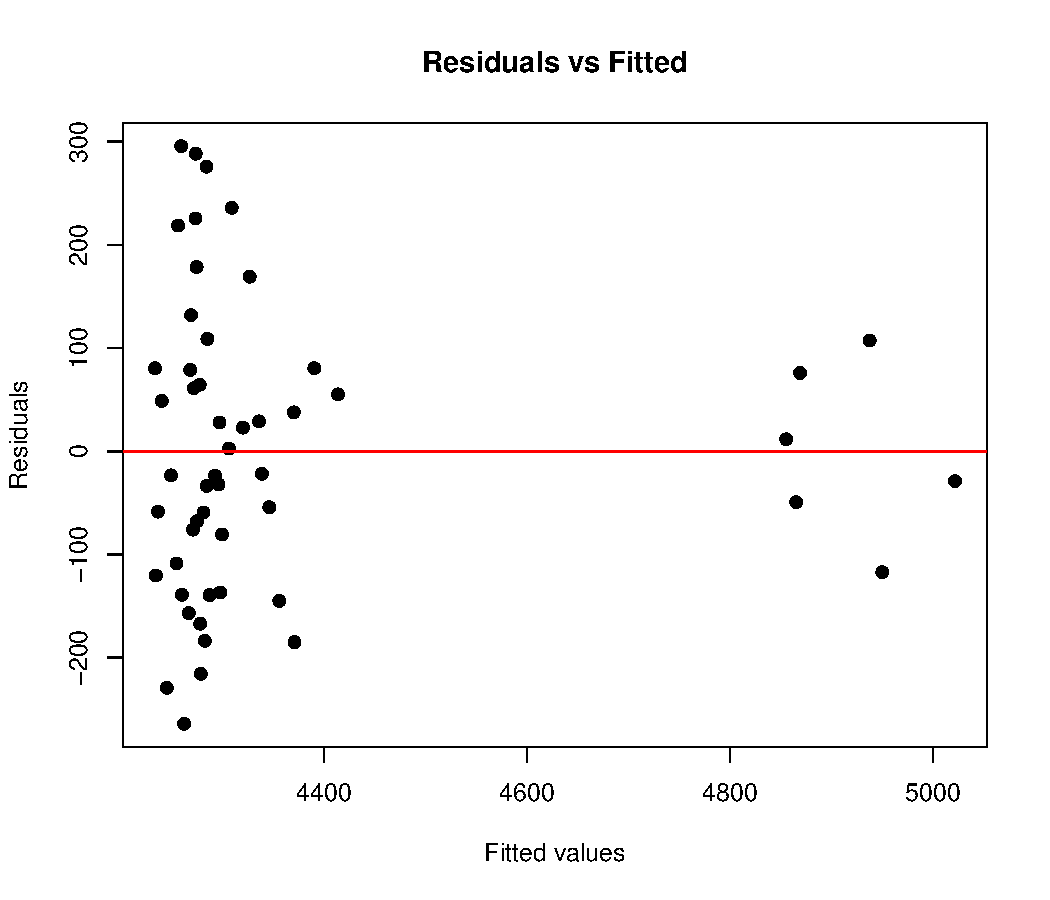
\includegraphics[keepaspectratio]{RMD_files/figure-latex/unnamed-chunk-11-1.pdf}}

\begin{Shaded}
\begin{Highlighting}[]
\FunctionTok{options}\NormalTok{(}\AttributeTok{repr.plot.width =} \DecValTok{7}\NormalTok{, }\AttributeTok{repr.plot.height =} \DecValTok{6}\NormalTok{)}
\CommentTok{\# Biểu đồ Standardized Residuals vs Fitted Values}
\FunctionTok{plot}\NormalTok{(result}\SpecialCharTok{$}\NormalTok{fitted.values, }\FunctionTok{rstandard}\NormalTok{(result),}
     \AttributeTok{main =} \StringTok{"Standardized Residuals vs Fitted"}\NormalTok{,}
     \AttributeTok{xlab =} \StringTok{"Fitted values"}\NormalTok{, }\AttributeTok{ylab =} \StringTok{"Standardized Residuals"}\NormalTok{,}
     \AttributeTok{pch =} \DecValTok{19}\NormalTok{)}
\FunctionTok{abline}\NormalTok{(}\AttributeTok{h =} \DecValTok{0}\NormalTok{, }\AttributeTok{col =} \StringTok{"red"}\NormalTok{)}
\end{Highlighting}
\end{Shaded}

\pandocbounded{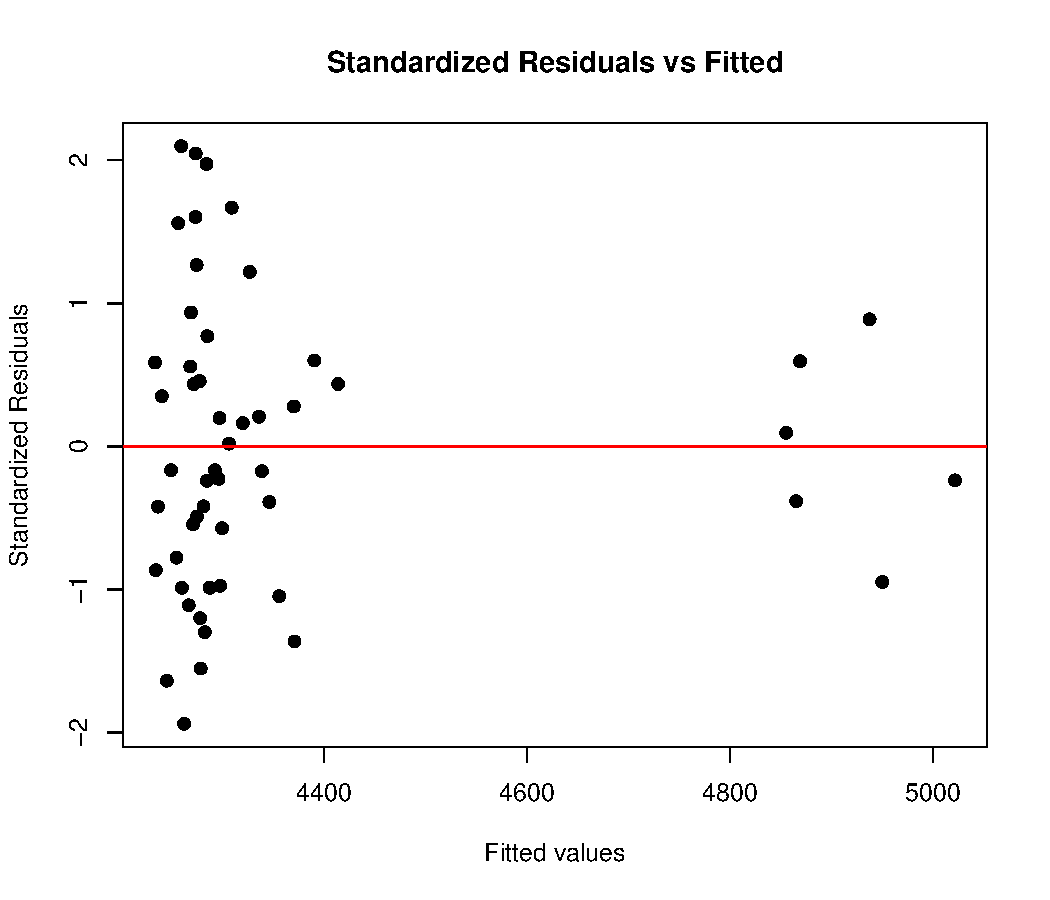
\includegraphics[keepaspectratio]{RMD_files/figure-latex/unnamed-chunk-12-1.pdf}}

\begin{Shaded}
\begin{Highlighting}[]
\FunctionTok{options}\NormalTok{(}\AttributeTok{repr.plot.width =} \DecValTok{7}\NormalTok{, }\AttributeTok{repr.plot.height =} \DecValTok{6}\NormalTok{)}
\CommentTok{\# Biểu đồ Studentized Residuals vs Fitted Values}
\FunctionTok{plot}\NormalTok{(result}\SpecialCharTok{$}\NormalTok{fitted.values, }\FunctionTok{rstudent}\NormalTok{(result),}
     \AttributeTok{main =} \StringTok{"Studentized Residuals vs Fitted"}\NormalTok{,}
     \AttributeTok{xlab =} \StringTok{"Fitted values"}\NormalTok{, }\AttributeTok{ylab =} \StringTok{"Studentized Residuals"}\NormalTok{,}
     \AttributeTok{pch =} \DecValTok{19}\NormalTok{)}
\FunctionTok{abline}\NormalTok{(}\AttributeTok{h =} \DecValTok{0}\NormalTok{, }\AttributeTok{col =} \StringTok{"red"}\NormalTok{)}
\end{Highlighting}
\end{Shaded}

\pandocbounded{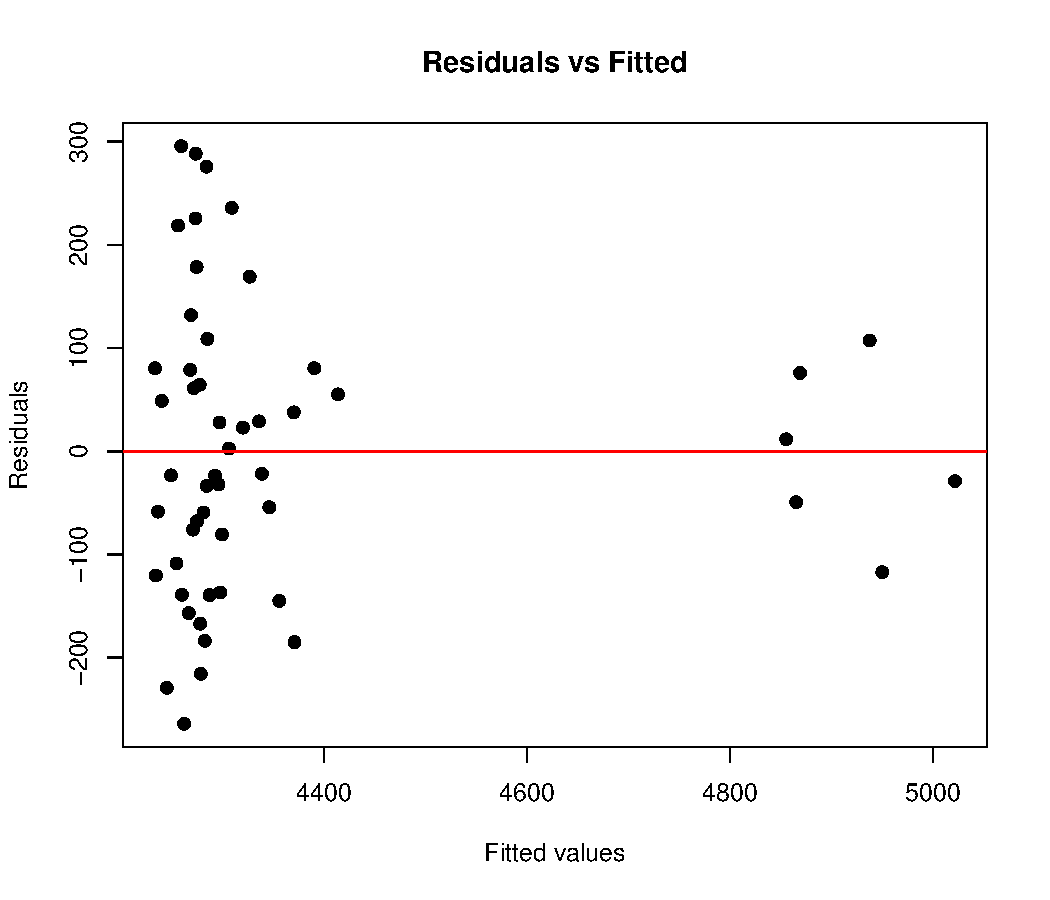
\includegraphics[keepaspectratio]{RMD_files/figure-latex/unnamed-chunk-13-1.pdf}}

\begin{Shaded}
\begin{Highlighting}[]
\CommentTok{\# Reset lại layout đồ họa về mặc định}
\FunctionTok{par}\NormalTok{(}\AttributeTok{mfrow =} \FunctionTok{c}\NormalTok{(}\DecValTok{1}\NormalTok{,}\DecValTok{1}\NormalTok{))}
\end{Highlighting}
\end{Shaded}

\subsection{Part 2}\label{part-2-1}

\begin{Shaded}
\begin{Highlighting}[]
\FunctionTok{library}\NormalTok{(readxl)}
\NormalTok{data }\OtherTok{\textless{}{-}} \FunctionTok{read\_excel}\NormalTok{(}\StringTok{"grocery.xlsx"}\NormalTok{, }\AttributeTok{col\_names =} \ConstantTok{TRUE}\NormalTok{)}

\CommentTok{\# Xây dựng mô hình hồi quy first order với các biến dự đoán: shipped, cost, và holiday}
\NormalTok{fit }\OtherTok{\textless{}{-}} \FunctionTok{lm}\NormalTok{(labor }\SpecialCharTok{\textasciitilde{}}\NormalTok{ shipped }\SpecialCharTok{+}\NormalTok{ cost }\SpecialCharTok{+}\NormalTok{ holiday, }\AttributeTok{data =}\NormalTok{ data)}

\CommentTok{\# Lấy số quan sát (n) và số biến dự báo (p)}
\NormalTok{n }\OtherTok{\textless{}{-}} \FunctionTok{nrow}\NormalTok{(data)}
\NormalTok{p }\OtherTok{\textless{}{-}} \FunctionTok{length}\NormalTok{(}\FunctionTok{coef}\NormalTok{(fit)) }\SpecialCharTok{{-}} \DecValTok{1}  \CommentTok{\# trừ đi hệ số intercept}

\CommentTok{\# Tính phần dư studentized (rstudent)}
\NormalTok{student.res }\OtherTok{\textless{}{-}} \FunctionTok{rstudent}\NormalTok{(fit)}

\CommentTok{\# {-}{-}{-} (a) Sắp xếp các phần dư studentized và in ra}
\NormalTok{sorted\_res }\OtherTok{\textless{}{-}} \FunctionTok{sort}\NormalTok{(student.res)}
\FunctionTok{print}\NormalTok{(}\StringTok{"Sorted studentized residuals:"}\NormalTok{)}
\CommentTok{\#\textgreater{} [1] "Sorted studentized residuals:"}
\FunctionTok{print}\NormalTok{(sorted\_res)}
\CommentTok{\#\textgreater{}          32          35          14          51          20           8 }
\CommentTok{\#\textgreater{} {-}1.99766654 {-}1.66686277 {-}1.57563574 {-}1.37470514 {-}1.30688333 {-}1.20529304 }
\CommentTok{\#\textgreater{}           7          47          31          37           9          16 }
\CommentTok{\#\textgreater{} {-}1.11220903 {-}1.04682238 {-}0.98793522 {-}0.98726030 {-}0.97317140 {-}0.94585538 }
\CommentTok{\#\textgreater{}          23          39          46          18          36          28 }
\CommentTok{\#\textgreater{} {-}0.86199416 {-}0.77401415 {-}0.56690329 {-}0.53946536 {-}0.48548061 {-}0.41694583 }
\CommentTok{\#\textgreater{}          13           4          21          12          48           1 }
\CommentTok{\#\textgreater{} {-}0.41516269 {-}0.38465346 {-}0.37866873 {-}0.23775605 {-}0.23443689 {-}0.22408724 }
\CommentTok{\#\textgreater{}           3          26          30          49          22          15 }
\CommentTok{\#\textgreater{} {-}0.17058921 {-}0.16427705 {-}0.16381817  0.01909697  0.09348669  0.16177701 }
\CommentTok{\#\textgreater{}           6          41          45          25          29          44 }
\CommentTok{\#\textgreater{}  0.19612403  0.20535372  0.27680521  0.34737819  0.43222641  0.43246959 }
\CommentTok{\#\textgreater{}          52          27          24           5          42          19 }
\CommentTok{\#\textgreater{}  0.45278959  0.55395260  0.58204380  0.59079243  0.59660183  0.76695374 }
\CommentTok{\#\textgreater{}          43          11           2          17          33          50 }
\CommentTok{\#\textgreater{}  0.88556630  0.93459516  1.22549009  1.27571169  1.58403006  1.63020460 }
\CommentTok{\#\textgreater{}          34          10          38          40 }
\CommentTok{\#\textgreater{}  1.70041654  2.03651764  2.11878596  2.17827186}

\CommentTok{\# Tính giá trị tới hạn theo phương pháp Bonferroni}
\CommentTok{\# Sử dụng α = 0.05. Giá trị tới hạn: qt(1 {-} α/(2*n), df = n {-} p {-} 1)}
\NormalTok{alpha }\OtherTok{\textless{}{-}} \FloatTok{0.05}
\NormalTok{crit }\OtherTok{\textless{}{-}} \FunctionTok{qt}\NormalTok{(}\DecValTok{1} \SpecialCharTok{{-}}\NormalTok{ alpha}\SpecialCharTok{/}\NormalTok{(}\DecValTok{2}\SpecialCharTok{*}\NormalTok{n), }\AttributeTok{df =}\NormalTok{ n }\SpecialCharTok{{-}}\NormalTok{ p }\SpecialCharTok{{-}} \DecValTok{1}\NormalTok{)}
\FunctionTok{print}\NormalTok{(}\StringTok{"Critical value (Bonferroni):"}\NormalTok{)}
\CommentTok{\#\textgreater{} [1] "Critical value (Bonferroni):"}
\FunctionTok{print}\NormalTok{(crit)}
\CommentTok{\#\textgreater{} [1] 3.518198}
\end{Highlighting}
\end{Shaded}

\begin{Shaded}
\begin{Highlighting}[]
\FunctionTok{options}\NormalTok{(}\AttributeTok{repr.plot.width =} \DecValTok{7}\NormalTok{, }\AttributeTok{repr.plot.height =} \DecValTok{6}\NormalTok{)}
\CommentTok{\# {-}{-}{-} (b) Vẽ biểu đồ phần dư studentized và overlay các đường giới hạn tới hạn}
\FunctionTok{plot}\NormalTok{(student.res, }
     \AttributeTok{ylab =} \StringTok{"Studentized Residuals"}\NormalTok{, }
     \AttributeTok{main =} \StringTok{"Studentized Residuals with Bonferroni Critical Lines"}\NormalTok{,}
     \AttributeTok{ylim =} \FunctionTok{c}\NormalTok{(}\SpecialCharTok{{-}}\DecValTok{4}\NormalTok{, }\DecValTok{4}\NormalTok{))}
\FunctionTok{abline}\NormalTok{(}\AttributeTok{h =}\NormalTok{ crit, }\AttributeTok{col =} \StringTok{"red"}\NormalTok{, }\AttributeTok{lty =} \DecValTok{2}\NormalTok{)}
\FunctionTok{abline}\NormalTok{(}\AttributeTok{h =} \SpecialCharTok{{-}}\NormalTok{crit, }\AttributeTok{col =} \StringTok{"red"}\NormalTok{, }\AttributeTok{lty =} \DecValTok{2}\NormalTok{)}
\end{Highlighting}
\end{Shaded}

\pandocbounded{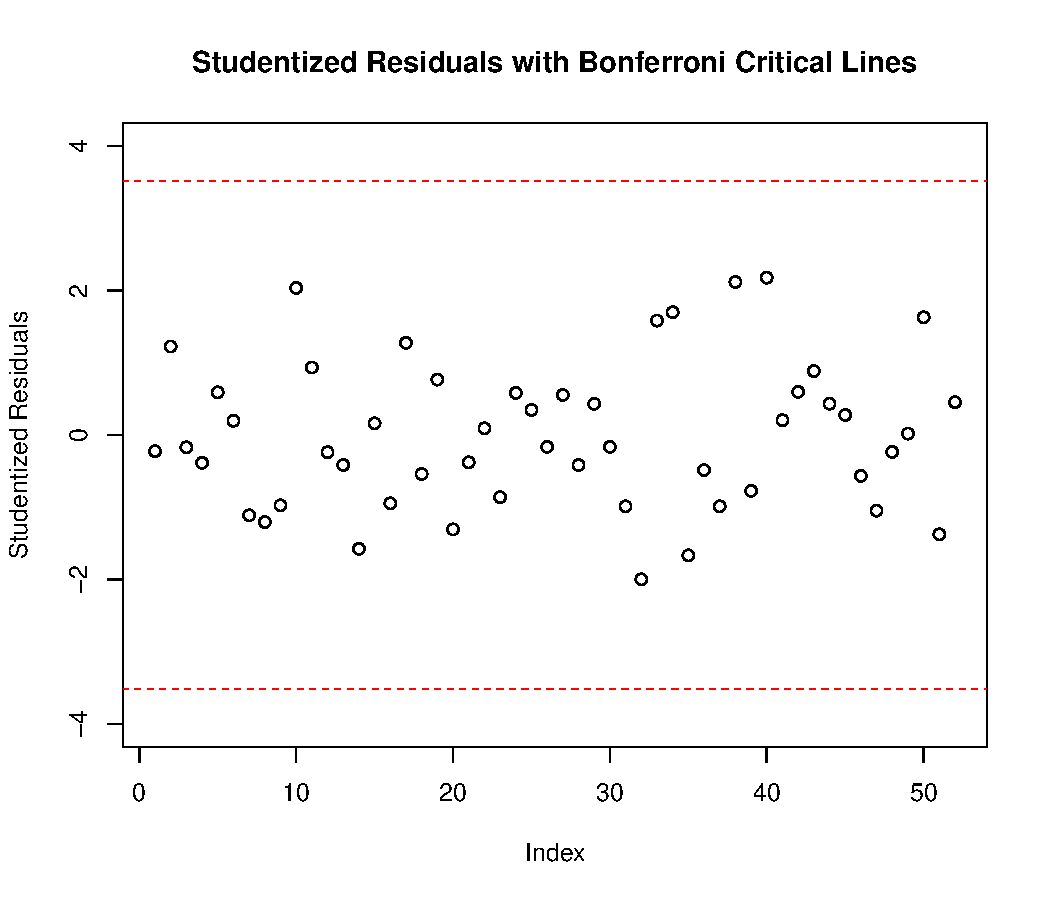
\includegraphics[keepaspectratio]{RMD_files/figure-latex/unnamed-chunk-16-1.pdf}}

\begin{Shaded}
\begin{Highlighting}[]
\CommentTok{\# {-}{-}{-} (c) Liệt kê các quan sát có |studentized residual| \textgreater{} giá trị tới hạn}
\NormalTok{outliers }\OtherTok{\textless{}{-}} \FunctionTok{which}\NormalTok{(}\FunctionTok{abs}\NormalTok{(student.res) }\SpecialCharTok{\textgreater{}}\NormalTok{ crit)}
\FunctionTok{print}\NormalTok{(}\StringTok{"Indices of potential outliers (|t\_i| \textgreater{} critical value):"}\NormalTok{)}
\CommentTok{\#\textgreater{} [1] "Indices of potential outliers (|t\_i| \textgreater{} critical value):"}
\FunctionTok{print}\NormalTok{(outliers)}
\CommentTok{\#\textgreater{} named integer(0)}
\end{Highlighting}
\end{Shaded}


\end{document}
